\documentclass[11pt,a4paper]{article}

\usepackage[utf8]{inputenc}
\usepackage[margin=1in]{geometry}
\usepackage{amsmath,amssymb,amsfonts,amsthm}
\usepackage{booktabs}
\usepackage{multirow}
\usepackage{graphicx}
\usepackage{hyperref}
\usepackage{microtype}
\usepackage{cite}
\usepackage{subcaption}
\usepackage{tikz}
\usetikzlibrary{shapes.geometric, arrows.meta, positioning, calc, fit}
\usepackage{pgfplots}
\pgfplotsset{compat=1.17}
\usepackage{xcolor}

\hypersetup{
    colorlinks=true,
    linkcolor=blue,
    citecolor=blue,
    urlcolor=blue
}

\newtheorem{proposition}{Proposition}
\setlength{\emergencystretch}{2em}
\renewcommand{\topfraction}{0.9}
\renewcommand{\dbltopfraction}{0.9}
\renewcommand{\textfraction}{0.07}
\renewcommand{\floatpagefraction}{0.75}
\renewcommand{\dblfloatpagefraction}{0.75}
\setcounter{topnumber}{3}
\setcounter{totalnumber}{5}

% Every result number quoted in the text is a macro generated from results/v2 by
% scripts/paper_v2_report.py. Tables in tables/v2_*.tex are generated by the same script.
% Generated by scripts/paper_v2_report.py -- do not edit by hand.
\newcommand{\vBbCnnETThOne}{+6.8}
\newcommand{\vBbCnnETThTwo}{+9.8}
\newcommand{\vBbCnnETTmOne}{+10.7}
\newcommand{\vBbCnnETTmTwo}{+21.1}
\newcommand{\vBbCnnElectricity}{+51.7}
\newcommand{\vBbCnnSolar}{+10.3}
\newcommand{\vBbCnnTraffic}{+43.4}
\newcommand{\vBbCnnWeather}{+16.5}
\newcommand{\vBbMlpETThOne}{+2.2}
\newcommand{\vBbMlpETThTwo}{\ensuremath{-}0.1}
\newcommand{\vBbMlpETTmOne}{\ensuremath{-}1.6}
\newcommand{\vBbMlpETTmTwo}{+3.2}
\newcommand{\vBbMlpElectricity}{+2.3}
\newcommand{\vBbMlpSolar}{\ensuremath{-}13.7}
\newcommand{\vBbMlpTraffic}{\ensuremath{-}0.3}
\newcommand{\vBbMlpWeather}{\ensuremath{-}8.1}
\newcommand{\vBbPatchBestCount}{5}
\newcommand{\vBbSorETThOne}{+6.1}
\newcommand{\vBbSorETThTwo}{+0.4}
\newcommand{\vBbSorETTmOne}{+0.6}
\newcommand{\vBbSorETTmTwo}{+4.1}
\newcommand{\vBbSorElectricity}{+7.8}
\newcommand{\vBbSorSolar}{\ensuremath{-}16.0}
\newcommand{\vBbSorTraffic}{+1.1}
\newcommand{\vBbSorWeather}{\ensuremath{-}6.4}
\newcommand{\vBestCycleFamily}{16}
\newcommand{\vBestFixed}{8}
\newcommand{\vBestPatch}{11}
\newcommand{\vBestTransform}{5}
\newcommand{\vCycleCells}{32}
\newcommand{\vCycleETThOne}{\ensuremath{-}0.22}
\newcommand{\vCycleETThTwo}{+3.18}
\newcommand{\vCycleETThTwoLevelShare}{60}
\newcommand{\vCycleETThTwoWorstH}{720}
\newcommand{\vCycleETTmOne}{\ensuremath{-}2.14}
\newcommand{\vCycleETTmTwo}{\ensuremath{-}3.65}
\newcommand{\vCycleElectricity}{\ensuremath{-}6.55}
\newcommand{\vCycleGainDailySlowShare}{75}
\newcommand{\vCyclePeriodComplete}{complete}
\newcommand{\vCycleSigBetter}{2}
\newcommand{\vCycleSigWorse}{0}
\newcommand{\vCycleSolar}{\ensuremath{-}3.56}
\newcommand{\vCycleTraffic}{\ensuremath{-}2.15}
\newcommand{\vCycleWeather}{\ensuremath{-}1.67}
\newcommand{\vCycleWins}{27}
\newcommand{\vDailyErFixedMax}{0.93}
\newcommand{\vDailyErFixedMin}{0.36}
\newcommand{\vDailyFvuFixedETThOne}{0.42}
\newcommand{\vDailyFvuFixedETThTwo}{0.61}
\newcommand{\vDailyFvuFixedETTmOne}{0.36}
\newcommand{\vDirtyRuns}{0}
\newcommand{\vDlinETThOneSevenTwenty}{0.4776}
\newcommand{\vDlinETThOneSevenTwentyStd}{0.0601}
\newcommand{\vDsofLinMaxAbs}{1.0}
\newcommand{\vDsofSorCtrlWorseMain}{7}
\newcommand{\vDsofSorHardBeatsMain}{3}
\newcommand{\vDsofSorHardEOneMax}{8.7}
\newcommand{\vDsofSorHardEOneMin}{2.2}
\newcommand{\vDsofSorHardETwoMax}{\ensuremath{-}0.5}
\newcommand{\vDsofSorHardETwoMin}{\ensuremath{-}5.8}
\newcommand{\vDsofStudentBeatsFixed}{3}
\newcommand{\vDsofStudentBeatsFixedWhere}{ETTh1, $H=192$; ETTh1, $H=720$; ETTh2, $H=336$}
\newcommand{\vDsofZeroGateMax}{83}
\newcommand{\vDsofZeroGateMin}{58}
\newcommand{\vFastEnergyPatchMax}{0.60}
\newcommand{\vFastEnergyPatchMin}{0.01}
\newcommand{\vFastErMedian}{0.22}
\newcommand{\vFastFvuCells}{544}
\newcommand{\vFastFvuFixedGtOne}{3}
\newcommand{\vFastFvuGtOne}{63}
\newcommand{\vFastFvuMax}{1.29}
\newcommand{\vFastFvuMedian}{0.85}
\newcommand{\vFastFvuMin}{0.35}
\newcommand{\vFastFvuPatchGtOne}{4}
\newcommand{\vFastFvuSnaiveMax}{2.02}
\newcommand{\vFastFvuSnaiveMin}{0.68}
\newcommand{\vFixedETThOneNinetySix}{0.3722}
\newcommand{\vFoundBoltBest}{1}
\newcommand{\vFoundCells}{32}
\newcommand{\vFoundMaxWindows}{120}
\newcommand{\vFoundMinWindows}{4}
\newcommand{\vFoundTfmBeatsFixed}{6}
\newcommand{\vFoundTimesfmBest}{4}
\newcommand{\vFoundTrainedBest}{27}
\newcommand{\vFourierBaseBeatsSnaive}{14}
\newcommand{\vFourierBoltCells}{32}
\newcommand{\vFourierBoltMedian}{+33}
\newcommand{\vFourierBoltWorse}{31}
\newcommand{\vFourierTfiveCells}{32}
\newcommand{\vFourierTfiveMedian}{+21}
\newcommand{\vFourierTfiveWorse}{19}
\newcommand{\vFourierTfmCells}{32}
\newcommand{\vFourierTfmMedian}{+29}
\newcommand{\vFourierTfmWorse}{32}
\newcommand{\vFourierTtmCells}{8}
\newcommand{\vFourierTtmMedian}{+69}
\newcommand{\vFourierTtmWorse}{6}
\newcommand{\vGpuList}{GeForce RTX 2070 SUPER (1025); RTX PRO 6000 Blackwell Max-Q Workstation Edition (384); RTX PRO 5000 Blackwell (287)}
\newcommand{\vIncompleteCells}{none}
\newcommand{\vLeadNaiveNeverBeaten}{never}
\newcommand{\vLeadRatioMax}{31.2}
\newcommand{\vLeadRatioMaxWhere}{Solar}
\newcommand{\vLeadRatioMin}{2.2}
\newcommand{\vLeadRatioMinWhere}{Traffic}
\newcommand{\vLevelShareETThOne}{16}
\newcommand{\vLevelShareETThTwo}{39}
\newcommand{\vLevelShareETTmTwo}{48}
\newcommand{\vLevelShareElectricity}{27}
\newcommand{\vLevelShareMax}{63}
\newcommand{\vLevelShareMin}{4}
\newcommand{\vLevelShareTraffic}{7}
\newcommand{\vLinOutlierCell}{ETTm2, $H=336$}
\newcommand{\vLinOutlierStd}{0.0233}
\newcommand{\vLrCells}{512}
\newcommand{\vMaxBlocks}{59}
\newcommand{\vMaxParseval}{6.7\times 10^{-16}}
\newcommand{\vMinBlocks}{3}
\newcommand{\vMissingModels}{none}
\newcommand{\vMixBestVal}{\ensuremath{-}6.5}
\newcommand{\vMixBestWhere}{Solar with the Linear backbone}
\newcommand{\vMixCells}{112}
\newcommand{\vMixDatasets}{7}
\newcommand{\vMixSigBetter}{1}
\newcommand{\vMixSigWorse}{5}
\newcommand{\vMixWins}{33}
\newcommand{\vMixWorstVal}{+19.4}
\newcommand{\vMixWorstWhere}{Traffic with the Linear backbone}
\newcommand{\vNumTests}{252}
\newcommand{\vNumTrainedModels}{17}
\newcommand{\vNumUntestable}{21}
\newcommand{\vOurDlinETThTwo}{0.3931}
\newcommand{\vParamCnnETThOne}{5,559}
\newcommand{\vParamCnnTraffic}{172,605}
\newcommand{\vParamLinETThOne}{32,534}
\newcommand{\vParamLinETThOneL}{242,822}
\newcommand{\vParamMlpETThOne}{221,974}
\newcommand{\vParamPatchETThOne}{81,742}
\newcommand{\vParamPatchTraffic}{922,908}
\newcommand{\vParamSorETThOne}{76,668}
\newcommand{\vPatchETThOneFast}{+33.2}
\newcommand{\vPatchETThOneTotal}{+9.2}
\newcommand{\vPatchElec}{+2.7}
\newcommand{\vPatchSigBetter}{1}
\newcommand{\vPatchSigWorse}{0}
\newcommand{\vPatchSolar}{\ensuremath{-}20.4}
\newcommand{\vPatchSolarDailyShare}{57}
\newcommand{\vPatchSolarLevelShare}{36}
\newcommand{\vPatchWeather}{\ensuremath{-}9.8}
\newcommand{\vPatchWeatherLevelShare}{83}
\newcommand{\vPatchWins}{20}
\newcommand{\vPeriodETTmTwoMaxAbs}{0.16}
\newcommand{\vPeriodElecMax}{8.9}
\newcommand{\vPeriodElecMin}{5.7}
\newcommand{\vPeriodElecSig}{3}
\newcommand{\vPeriodElecSlowDailyShare}{80}
\newcommand{\vPeriodElecSlowShare}{48}
\newcommand{\vPeriodIdentical}{identical to within $10^{-6}$}
\newcommand{\vPeriodSameCount}{5}
\newcommand{\vPeriodSameList}{ETTh1, ETTh2, ETTm1, Weather, Solar}
\newcommand{\vPeriodSigBetter}{0}
\newcommand{\vPeriodTests}{12}
\newcommand{\vPeriodTrafficSevenTwenty}{\ensuremath{-}1.29}
\newcommand{\vPeriodTrafficSevenTwentySig}{not significant}
\newcommand{\vPubCells}{28}
\newcommand{\vPubDlinETThTwo}{0.605}
\newcommand{\vPubPatchMedAbs}{1.3}
\newcommand{\vPubPatchWithinFive}{24}
\newcommand{\vRankCNN}{15.95}
\newcommand{\vRankDLinear}{8.91}
\newcommand{\vRankFixed}{5.19}
\newcommand{\vRankLinear}{9.81}
\newcommand{\vRankPatch}{3.91}
\newcommand{\vRankProLin}{8.84}
\newcommand{\vRankProLinCI}{5.91}
\newcommand{\vRankProMlpCI}{5.31}
\newcommand{\vRankTransformLinear}{4.75}
\newcommand{\vRunsExpected}{1696}
\newcommand{\vRunsFinal}{1696}
\newcommand{\vRunsLrsel}{2328}
\newcommand{\vRunsMissing}{0}
\newcommand{\vSkillCells}{544}
\newcommand{\vSkillFixedETThOne}{0.30}
\newcommand{\vSkillFixedETThTwo}{0.26}
\newcommand{\vSkillFixedETTmOne}{0.27}
\newcommand{\vSkillFixedETTmTwo}{0.30}
\newcommand{\vSkillFixedElectricity}{0.52}
\newcommand{\vSkillFixedSolar}{0.26}
\newcommand{\vSkillFixedTraffic}{0.63}
\newcommand{\vSkillFixedWeather}{0.35}
\newcommand{\vSkillMaxFixed}{0.67}
\newcommand{\vSkillMinFixed}{0.20}
\newcommand{\vSkillNeg}{1}
\newcommand{\vSkillNegWhere}{Pro-CNN on ETTh2, $H=96$}
\newcommand{\vSlowFvuFixedMax}{1.08}
\newcommand{\vSlowFvuFixedMin}{0.50}
\newcommand{\vTeacherETThOneNinetySix}{0.3950}
\newcommand{\vTeacherWorseThanFixed}{7}
\newcommand{\vTrDbfourMean}{\ensuremath{-}0.18}
\newcommand{\vTrDbfourMedian}{\ensuremath{-}0.12}
\newcommand{\vTrDbfourRank}{4.44}
\newcommand{\vTrDbfourWins}{19}
\newcommand{\vTrDctMean}{\ensuremath{-}0.79}
\newcommand{\vTrDctMedian}{\ensuremath{-}0.33}
\newcommand{\vTrDctRank}{2.53}
\newcommand{\vTrDctSigBetter}{5}
\newcommand{\vTrDctSigWorse}{0}
\newcommand{\vTrDctWins}{24}
\newcommand{\vTrDlinMean}{+0.02}
\newcommand{\vTrDlinMedian}{\ensuremath{-}0.12}
\newcommand{\vTrDlinRank}{3.62}
\newcommand{\vTrDlinWins}{23}
\newcommand{\vTrHaarMean}{\ensuremath{-}0.34}
\newcommand{\vTrHaarMedian}{\ensuremath{-}0.16}
\newcommand{\vTrHaarRank}{3.62}
\newcommand{\vTrHaarWins}{25}
\newcommand{\vTrRfftBestCell}{ETTm2, $H=336$}
\newcommand{\vTrRfftBestGain}{7.2}
\newcommand{\vTrRfftMean}{\ensuremath{-}0.67}
\newcommand{\vTrRfftMedian}{\ensuremath{-}0.30}
\newcommand{\vTrRfftRank}{2.41}
\newcommand{\vTrRfftSigBetter}{5}
\newcommand{\vTrRfftSigWorse}{0}
\newcommand{\vTrRfftWins}{25}
\newcommand{\vTrStftMean}{+3.01}
\newcommand{\vTrStftMedian}{+1.95}
\newcommand{\vTrStftRank}{6.62}
\newcommand{\vTrStftWins}{4}
\newcommand{\vUntestableWhere}{ETTh1 $H=720$, ETTh2 $H=720$, Traffic $H=720$}
\newcommand{\vXmAgree}{311}
\newcommand{\vXmCells}{312}
\newcommand{\vXmGpu}{GeForce RTX 4050 Laptop GPU}
\newcommand{\vXmMaxRel}{2.79}
\newcommand{\vXmMedRel}{0.000}
\newcommand{\vXmRuns}{866}


\title{\textbf{When Does Periodic and Frequency-Domain Modelling Help Lightweight Forecasting?\\A Controlled, Multi-Seed Evaluation of Automated CycleNet}}

\author{
    \textbf{Aaditya Chaturvedi}\\
    Information Systems and Machine Learning Lab (ISMLL)\\
    Institute for Computer Science, University of Hildesheim, Germany\\
    \texttt{chaturvedia@uni-hildesheim.de}
}

\date{\today}

\begin{document}

\maketitle

\begin{abstract}
We ask when frequency-domain and periodic modelling actually help lightweight multivariate time-series (MTS) forecasting, and when they fail. We study \textbf{Automated CycleNet} (CycleNet-Pro), which extends CycleNet's learnable recurrent cycles with (i)~automatic period discovery from the training data (FFT peak ranking, an autocorrelation significance filter and a multi-cycle gain test), (ii)~an automatically enabled cross-channel mixer, and (iii)~four residual backbones (Linear, MLP, 1D-CNN, SORMixer). All models, baselines and ablations are re-run in one controlled harness: identical data pipeline, trainer and evaluator, look-back $L=336$, $H\in\{96,192,336,720\}$, eight datasets, three seeds, validation-only learning-rate selection, and all stride-1 test windows (\vRunsFinal{} of \vRunsExpected{} pre-registered runs complete). Errors are decomposed exactly (Parseval) into level, slow ($T>36$\,h), daily ($8$--$36$\,h) and fast ($T<8$\,h) components. Four findings answer the question. (1)~\emph{The recurrent cycle itself helps}: with the known period it lowers MSE relative to an otherwise identical linear model in \vCycleWins{} of \vCycleCells{} dataset--horizon cells (largest on Electricity, \vCycleElectricity\% on average), and the gain comes mostly from the daily and slow bands. It fails on ETTh2 (\vCycleETThTwo\%), where the extra error is mostly a misplaced window mean. (2)~\emph{The automation does not help}: period discovery reproduces the known period on \vPeriodSameCount{} of 8 datasets (results identical to within $10^{-6}$), and where it differs it either changes little or costs accuracy (Electricity: a 24-step instead of a 168-step cycle, $+\vPeriodElecMin$ to $+\vPeriodElecMax$\% MSE). The automatic channel mixer beats forced channel independence in only \vMixWins{} of \vMixCells{} comparisons. (3)~\emph{Frequency-domain inputs do not change what a linear forecaster can express}: rFFT, DCT, Haar-DWT and DLinear inputs give the same hypothesis class as raw inputs, and their measured effects are below one percent on average (rFFT \vTrRfftMean\%, DCT \vTrDctMean\%). (4)~\emph{Diagnostics}: \vLevelShareMin--\vLevelShareMax\% of a trained model's MSE is level error, and the fast band is largely unpredictable (median $FVU_{\text{fast}}=\vFastFvuMedian$). A re-run PatchTST has the best mean rank among the \vNumTrainedModels{} trained models (\vRankPatch); zero-shot foundation models are beaten by a trained model in \vFoundTrainedBest{} of \vFoundCells{} cells on identical windows.
\end{abstract}

\section{Introduction}
\label{sec:intro}
Long-horizon multivariate forecasting is dominated by two families: attention-based models~\cite{wu2021autoformer, zhou2022fedformer, nie2023patchtst} and lightweight linear or decomposition models that match them at a fraction of the cost~\cite{zeng2023dlinear}. Many recent lightweight models add an explicit frequency or periodic component, for example learnable recurrent cycles in CycleNet~\cite{liu2024cyclenet} or frequency-domain representations in FEDformer~\cite{zhou2022fedformer} and wavelet mixers~\cite{wpmixer2024}. The research question set with the supervisor of this project is:
\begin{quote}
\emph{When does frequency-domain modelling actually help versus fail in lightweight MTS forecasting?}
\end{quote}
Answering it needs two things that aggregate leaderboard numbers do not provide: controlled contrasts that change one component at a time, and a diagnostic that says on which time scale a model gains or loses accuracy.

This paper reports a controlled re-run of every experiment of the project (the ``v2'' protocol). An earlier draft of this paper used single-seed results from several separate training scripts, mixed published baselines run at a different look-back into the same table, and read diagnostic metrics that were later found to be mis-defined. Appendix~\ref{app:reconciliation} lists what changed and why. All numbers below come from one harness and are regenerated from the result files by a single script.

\paragraph{Contributions.}
\begin{itemize}
    \item \textbf{Automated CycleNet (CycleNet-Pro)}, the model under study: CycleNet's recurrent cycles with automatic period discovery, an automatic channel-mixing decision and four interchangeable residual backbones (Section~\ref{sec:cyclenet}).
    \item \textbf{A controlled benchmark}: \vNumTrainedModels{} trained models and two naive references on eight datasets, four horizons and three seeds in one harness, with validation-only learning-rate selection, provenance in every result file, a cross-machine reproduction check, and equal-accuracy tests (batch-means variance, Holm correction) for every comparison we claim (Section~\ref{sec:protocol}).
    \item \textbf{Component-level answers} to the research question: the recurrent cycle, the period discovery, the channel mixer, the backbone and the input transform are each isolated by a dedicated contrast (Sections~\ref{sec:res-cycle}--\ref{sec:res-transform}).
    \item \textbf{A corrected spectral diagnostic}: an exact Parseval split of MSE into a level term and three bands defined by period in real time, with interpretation rules that do not mistake unpredictable content for model failure (Sections~\ref{sec:diagnostics} and~\ref{sec:res-bands}).
    \item \textbf{Two frequency-motivated extensions tested under the same protocol}: Fourier decoupling for zero-shot foundation models and spectral distillation (DSOF-SD) into lightweight students (Sections~\ref{sec:res-foundation}--\ref{sec:res-dsof}).
\end{itemize}

\section{Related Work}
\label{sec:related_work}

\paragraph{Lightweight linear models versus Transformers.}
Autoformer~\cite{wu2021autoformer} introduced auto-correlation attention and FEDformer~\cite{zhou2022fedformer} attention in the Fourier and wavelet domains. PatchTST~\cite{nie2023patchtst} uses channel-independent attention over patches, and HDMixer~\cite{hdmixer2024} extendable patches with hierarchical mixing. DLinear~\cite{zeng2023dlinear} showed that a linear map on a moving-average trend/seasonal split can match these models. Reversible instance normalisation (RevIN)~\cite{kim2021revin} is widely used to counter distribution shift between look-back and horizon.

\paragraph{Explicit periodicity.}
CycleNet~\cite{liu2024cyclenet} learns one table per channel indexed by the phase of a known cycle length, subtracts it from the input and adds it to the forecast; its successor TQNet~\cite{lin2025tqnet} adds temporal queries for inter-variable dependencies. FreqCycle~\cite{FreqCycle2026} and FreqLens~\cite{FreqLens2026} argue that time-domain training under-weights mid and high frequencies. Our work keeps CycleNet's mechanism and asks whether making its cycle length and channel handling automatic helps.

\paragraph{Spectral and wavelet representations.}
WPMixer~\cite{wpmixer2024} mixes wavelet-packet subbands and WaveMoE~\cite{WaveMoE2026} routes tokens over wavelet subbands. We do not add a new spectral module; we compare input transforms under a fixed linear head and use Parseval's identity to locate errors by time scale.

\paragraph{Foundation models and fair benchmarking.}
Zero-shot forecasters such as TimesFM~\cite{das2024timesfm}, Chronos~\cite{ansari2024chronos} and Tiny Time Mixers~\cite{ekambaram2024ttm} are pre-trained on large corpora. TFB~\cite{qiu2024tfb} documents benchmark pitfalls such as dropping the last incomplete test batch, which we avoid. Following standard forecasting practice~\cite{hyndman2021fpp3}, we report skill against a seasonal-naive forecast, and we test claimed differences for equal expected loss in the spirit of Diebold and Mariano~\cite{diebold1995comparing}, with a variance estimate suited to overlapping forecast windows.

\section{Diagnostic Apparatus: Exact Band Decomposition}
\label{sec:diagnostics}

\subsection{Setup}
Let $\mathbf{X}\in\mathbb{R}^{L\times C}$ be the look-back window and $\mathbf{Y}\in\mathbb{R}^{H\times C}$ the target. All metrics are computed on the full stride-1 test set, in the space of the training-split standard scaler, and averaged over windows and channels.

\subsection{Parseval split of MSE}
For one window and channel let $e(t)=y(t)-\hat y(t)$, $t=0,\dots,H-1$, and $E(k)$ its DFT. With the one-sided rFFT ($M=\lfloor H/2\rfloor+1$ bins) and weights $w_0=1$, $w_{H/2}=1$ for even $H$, and $w_k=2$ otherwise, Parseval's identity gives
\begin{equation}
\frac{1}{H}\sum_{t=0}^{H-1} e(t)^2 \;=\; \frac{1}{H^2}\sum_{k=0}^{M-1} w_k\,|E(k)|^2 .
\end{equation}
We assign every bin to one component by its period in real time, $T_k = \Delta t\cdot H/k$, where $\Delta t$ is the sampling interval (1\,h for ETTh1/2, Electricity and Traffic; 15\,min for ETTm1/2; 10\,min for Weather and Solar):
\begin{equation}
\underbrace{k=0}_{\text{level}},\qquad
\underbrace{T_k>36\,\text{h}}_{\text{slow}},\qquad
\underbrace{8\,\text{h}\le T_k\le 36\,\text{h}}_{\text{daily}},\qquad
\underbrace{T_k<8\,\text{h}}_{\text{fast}} .
\end{equation}
The level term is the squared error of the window mean. The slow band holds trend, multi-day and weekly variation (a 168\,h cycle is ``slow''), the daily band the 24\,h cycle and its 12\,h harmonic, and the fast band intra-day fluctuation. By construction
\begin{equation}
\text{MSE} = \text{MSE}_{\text{level}} + \text{MSE}_{\text{slow}} + \text{MSE}_{\text{daily}} + \text{MSE}_{\text{fast}},
\end{equation}
and the largest violation over all \vRunsFinal{} runs is $\vMaxParseval$. A band exists only if the window resolves it: the slow band is empty when $H\Delta t\le 36$\,h (ETTm1/2 at $H=96$; Weather and Solar at $H\in\{96,192\}$), and when the window is shorter than a day (Weather and Solar at $H=96$, 16\,h) the 24\,h cycle itself is not resolved and the daily band holds only the 16\,h and 8\,h bins. Empty bands are shown as ``--''.

\subsection{Interpretation rules}
For band $b\in\{\text{slow},\text{daily},\text{fast}\}$ we report
\begin{equation}
FVU_b = \frac{\sum_{k\in b} w_k|E(k)|^2}{\sum_{k\in b} w_k|Y(k)|^2},\qquad
\rho_b = \frac{\sum_{k\in b} w_k|\hat Y(k)|^2}{\sum_{k\in b} w_k|Y(k)|^2},
\end{equation}
both summed over windows and channels; the level term has no FVU. A forecast that predicts nothing in a band (zero content there) has $FVU_b=1$. For content that cannot be predicted this is the \emph{correct} answer: an MSE-optimal forecast of an unpredictable band scores $FVU_b\approx 1$. We therefore read only $FVU_b$ clearly below 1 (the model captures real structure) or clearly above 1 (the model adds content with the wrong phase or amplitude) as informative, and never call $FVU_b\approx1$ a failure by itself. The energy ratio $\rho_b<1$ means the forecast is smoother than the truth, which is expected under squared loss; it is descriptive, not a score.

\subsection{Skill and lead time}
Skill against the seasonal-naive forecast (repeat the last day of the look-back) is $1-\text{MSE}_{\text{model}}/\text{MSE}_{\text{snaive}}$; values above 0 beat naive~\cite{hyndman2021fpp3}. We also record MSE at each lead step $1,\dots,H$. The diagnostics used in the earlier draft (fixed $0.1/0.4$ cycles-per-step bands, log-spectral distance, a rolling ``failure rate'') are not used; Appendix~\ref{app:reconciliation} explains why.

\begin{figure*}[t]
\centering
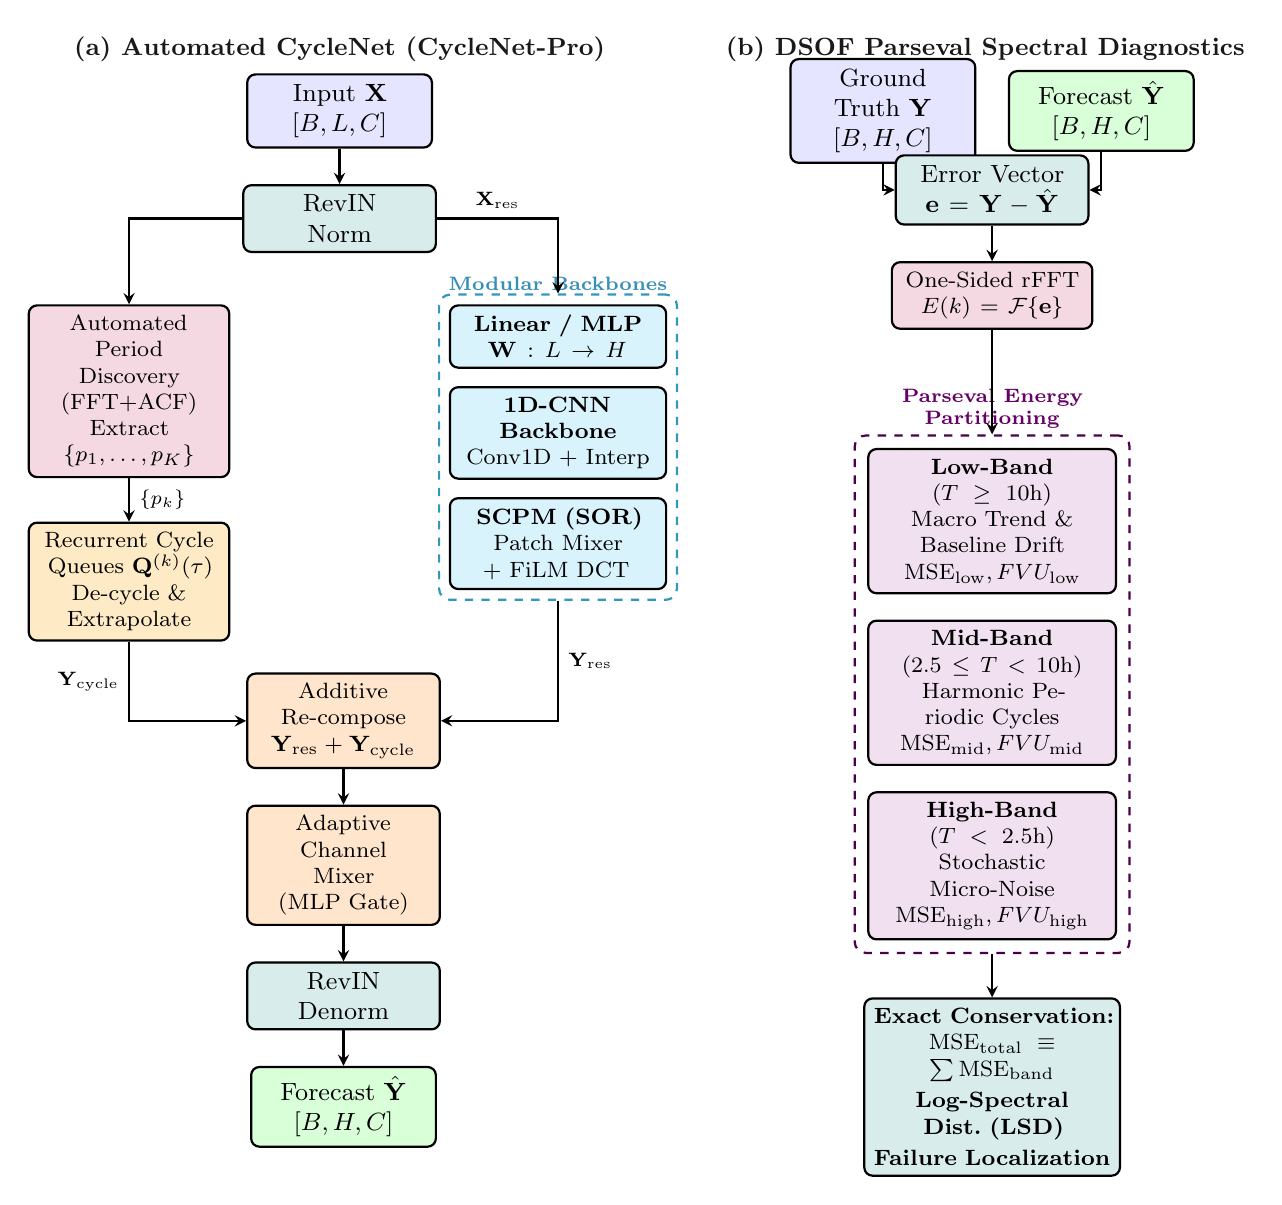
\begin{tikzpicture}[
    >=stealth,
    node distance=0.55cm and 0.55cm,
    font=\small,
    box/.style={draw, rounded corners=3pt, thick, align=center, inner sep=3.5pt, fill=white, font=\small},
    input/.style={box, fill=blue!10, text width=2.1cm},
    proc/.style={box, fill=teal!15, text width=2.2cm},
    period/.style={box, fill=purple!15, text width=2.3cm, font=\footnotesize},
    queue/.style={box, fill=yellow!30!orange!20, text width=2.3cm, font=\footnotesize},
    bb_node/.style={box, fill=cyan!15, text width=2.5cm, font=\footnotesize},
    mixer/.style={box, fill=orange!20, text width=2.2cm, font=\footnotesize},
    output/.style={box, fill=green!15, text width=2.1cm},
    diag/.style={box, fill=violet!12, text width=2.9cm, font=\footnotesize}
]

% =========================================================================
% PANEL (A): Proposed Architecture: Automated CycleNet (CycleNet-Pro)
% =========================================================================
\begin{scope}[local bounding box=panel_a]
    % Title centered above Column (A)
    \node[font=\bfseries\small, text=black!90, anchor=center] (title_a) at (3.0, 0.2) {(a) Automated CycleNet (CycleNet-Pro)};

    % Main vertical sequence (centered at x = 3.0cm)
    \node[input, below=0.5cm of title_a, anchor=center] (in) {Input $\mathbf{X}$\\$[B, L, C]$};
    \node[proc, below=0.45cm of in] (revin) {RevIN\\Norm};

    % Left: Periodic Branch
    \node[period, below left=0.65cm and 0.15cm of revin] (period_det) {Automated Period\\Discovery (FFT+ACF)\\Extract $\{p_1, \dots, p_K\}$};
    \node[queue, below=0.55cm of period_det] (cycle_q) {Recurrent Cycle\\Queues $\mathbf{Q}^{(k)}(\tau)$\\De-cycle \& Extrapolate};

    % Right: Modular Residual Backbones
    \node[bb_node, below right=0.65cm and 0.15cm of revin] (bb_lin) {\textbf{Linear / MLP}\\$\mathbf{W}: L \to H$};
    \node[bb_node, below=0.22cm of bb_lin] (bb_cnn) {\textbf{1D-CNN Backbone}\\Conv1D + Interp};
    \node[bb_node, below=0.22cm of bb_cnn] (bb_sor) {\textbf{SCPM (SOR)}\\Patch Mixer + FiLM DCT};

    % Dashed box around backbones
    \node[draw=cyan!75!black, dashed, thick, rounded corners=4pt, fit=(bb_lin) (bb_cnn) (bb_sor), inner sep=3.5pt] (bb_box) {};
    \node[font=\scriptsize\bfseries, text=cyan!70!black, anchor=south, fill=white, inner sep=1pt] at (bb_box.north) {Modular Backbones};

    % Merging Point
    \path (cycle_q.south) -- (bb_box.south) coordinate[midway] (merge_mid);
    
    \node[mixer, below=0.65cm of merge_mid] (add_node) {Additive Re-compose\\$\mathbf{Y}_{\text{res}} + \mathbf{Y}_{\text{cycle}}$};
    \node[mixer, below=0.45cm of add_node] (chan_mix) {Adaptive Channel\\Mixer (MLP Gate)};
    \node[proc, below=0.45cm of chan_mix] (denorm) {RevIN\\Denorm};
    \node[output, below=0.45cm of denorm] (out) {Forecast $\hat{\mathbf{Y}}$\\$[B, H, C]$};

    % Panel (A) Connectors
    \draw[->, thick] (in) -- (revin);
    
    % Flow to Periodic Branch
    \draw[->, thick] (revin) -| (period_det.north);
    \draw[->, thick] (period_det) -- (cycle_q) node[midway, right] {\scriptsize $\{p_k\}$};
    
    % Flow to Residual Branch
    \draw[->, thick] (revin) -| (bb_box.north) node[near start, above] {\scriptsize $\mathbf{X}_{\text{res}}$};
    
    % Flow to Re-composition
    \draw[->, thick] (cycle_q.south) |- (add_node.west) node[near start, left] {\scriptsize $\mathbf{Y}_{\text{cycle}}$};
    \draw[->, thick] (bb_box.south) |- (add_node.east) node[near start, right] {\scriptsize $\mathbf{Y}_{\text{res}}$};
    
    \draw[->, thick] (add_node) -- (chan_mix);
    \draw[->, thick] (chan_mix) -- (denorm);
    \draw[->, thick] (denorm) -- (out);
\end{scope}

% =========================================================================
% PANEL (B): Diagnostic Framework: DSOF Parseval Spectral Decomposition
% =========================================================================
\begin{scope}[shift={(8.0, 0)}, local bounding box=panel_b]
    % Title centered above Column (B) with clear horizontal clearance from Title (A)
    \node[font=\bfseries\small, text=black!90, anchor=center] (title_b) at (3.2, 0.2) {(b) DSOF Parseval Spectral Diagnostics};

    % Inputs at top
    \node[input, below=0.5cm of title_b, xshift=-1.3cm, anchor=center] (gt) {Ground Truth $\mathbf{Y}$\\$[B, H, C]$};
    \node[output, right=0.4cm of gt] (pred) {Forecast $\hat{\mathbf{Y}}$\\$[B, H, C]$};

    \path (gt) -- (pred) coordinate[midway] (input_mid);

    % Error sequence & rFFT
    \node[proc, below=0.55cm of input_mid] (err) {Error Vector\\$\mathbf{e} = \mathbf{Y} - \hat{\mathbf{Y}}$};
    \node[period, below=0.45cm of err, text width=2.3cm] (rfft) {One-Sided rFFT\\$E(k) = \mathcal{F}\{\mathbf{e}\}$};

    % Vertically Stacked Physical Subbands with generous 1.5cm clearance below rFFT
    \node[diag, below=1.5cm of rfft] (low) {\textbf{Low-Band} ($T \ge 10\text{h}$)\\Macro Trend \& Baseline Drift\\$\text{MSE}_{\text{low}}, FVU_{\text{low}}$};
    \node[diag, below=0.32cm of low] (mid) {\textbf{Mid-Band} ($2.5 \le T < 10\text{h}$)\\Harmonic Periodic Cycles\\$\text{MSE}_{\text{mid}}, FVU_{\text{mid}}$};
    \node[diag, below=0.32cm of mid] (high) {\textbf{High-Band} ($T < 2.5\text{h}$)\\Stochastic Micro-Noise\\$\text{MSE}_{\text{high}}, FVU_{\text{high}}$};

    % Enclosing box for Subbands
    \node[draw=violet!60!black, dashed, thick, rounded corners=4pt, fit=(low) (mid) (high), inner sep=4.5pt] (subband_box) {};
    
    % Group Label cleanly wrapped on two lines without touching the incoming arrow
    \node[font=\scriptsize\bfseries, text=violet!80!black, align=center, text width=2.5cm, anchor=south, fill=white, inner sep=2pt] at (subband_box.north) {Parseval Energy\\Partitioning};

    % Diagnostic Output Summary
    \node[proc, below=0.55cm of subband_box, text width=3.0cm, font=\footnotesize] (diag_out) {
        \textbf{Exact Conservation:}\\
        $\text{MSE}_{\text{total}} \equiv \sum \text{MSE}_{\text{band}}$\\[2pt]
        \textbf{Log-Spectral Dist.~(LSD)}\\[2pt]
        \textbf{Failure Localization}
    };

    % Panel (B) Connectors
    \draw[->, thick] (gt) |- (err);
    \draw[->, thick] (pred) |- (err);
    \draw[->, thick] (err) -- (rfft);
    
    % Arrow entering subband box cleanly
    \draw[->, thick] (rfft.south) -- (subband_box.north);
    \draw[->, thick] (subband_box.south) -- (diag_out);
\end{scope}

\end{tikzpicture}

\caption{\textbf{(a) Automated CycleNet (CycleNet-Pro).} Periods are discovered once from the training split. The learned cycles are subtracted from the RevIN-normalised look-back, a backbone maps the residual to the horizon, the cycles are added back, an optional channel mixer is applied, and RevIN is reversed. \textbf{(b) Diagnostics.} The forecast error is split exactly into a level term and slow, daily and fast bands defined by period in hours.}
\label{fig:architectures}
\end{figure*}

\section{Automated CycleNet (CycleNet-Pro)}
\label{sec:cyclenet}
This section describes the implementation that produced every CycleNet-Pro result (\nolinkurl{models/cyclenet/cyclenet_pro_Full.py}, used unchanged by the harness).

\subsection{Period discovery}
Discovery runs once per dataset on the mean over channels of the raw training split, $x$ (length $N$):
\begin{enumerate}
    \item \textbf{FFT candidates.} After removing the mean, the five largest local maxima of the rFFT power spectrum with periods in $[2,\min(L,N/2)]$ are converted to integer periods. Periods within $\max(2, 0.12\,p)$ of a stronger one are merged (spectral leakage).
    \item \textbf{ACF filter.} A candidate $p$ is kept if $|\text{ACF}(p)|>1.96/\sqrt{N}$, the 95\% white-noise bound. Survivors are ranked by $|\text{ACF}(p)|$.
    \item \textbf{Multi-cycle gain test.} Using the first $k\le 3$ periods, the series is reconstructed from the first 20 harmonics of each period and the variance reduction $R_k$ (in \% of $\mathrm{Var}(x)$) is computed. Period $k+1$ is added only if $R_{k+1}-R_k\ge 2$ percentage points.
\end{enumerate}
If no period survives, the strongest candidate (or 24) is used. The discovered periods are stored in every result file; Table~\ref{tab:period} lists them.

\subsection{Recurrent cycles}
For each period $p_k$ the model keeps a learnable table $\mathbf{Q}^{(k)}\in\mathbb{R}^{p_k\times C}$, initialised to zero. With $\tau$ the absolute time index of the first look-back step,
\begin{equation}
\mathbf{X}_{\text{res}} = \mathrm{RevIN}(\mathbf{X}) - \sum_k \mathbf{Q}^{(k)}_{(\tau+t)\bmod p_k},\quad t=0,\dots,L-1,
\end{equation}
and after the backbone the cycles are added back over the horizon, $\mathbf{Y}_{\text{pred}} = \mathbf{Y}_{\text{res}} + \sum_k \mathbf{Q}^{(k)}_{(\tau+L+t)\bmod p_k}$, $t=0,\dots,H-1$. RevIN here has a learnable per-channel affine map.

\subsection{Residual backbones}
All backbones are shared across channels.
\begin{itemize}
    \item \textbf{Linear}: one map $\mathbb{R}^{L}\to\mathbb{R}^{H}$ (the original CycleNet backbone).
    \item \textbf{MLP}: $L\to512\to H$ with GELU.
    \item \textbf{1D-CNN}: two Conv1D layers (kernel 5, width 32, GELU) applied along time with weights shared over time and channels, parameter-free linear interpolation from $L$ to $H$ steps, and a $1\times1$ convolution head. Its size does not depend on $L$ or $H$.
    \item \textbf{SORMixer}: two branches whose outputs are summed with learnable weights and a learnable scale. The \emph{DCT branch} applies an orthonormal DCT-II to the residual, multiplies two equal halves of the coefficient axis by learnable gains, inverts the DCT and maps the result to the horizon with an MLP ($L\to64\to H$). The \emph{overlap-patch branch} embeds patches of length 16 (stride 8) into 64 dimensions, mixes each patch with its two neighbours through an MLP, applies a sigmoid-gated tanh update, pools patches with learned softmax weights and projects to $H$ (dropout 0.1).
\end{itemize}

\subsection{Automatic channel mixing}
From the training split the model computes the mean absolute Pearson correlation between channels ($\bar r$), the mean of the maximum absolute lagged cross-correlation over lags up to 50 ($\bar m$), and the fraction of channel pairs with maximum lagged correlation above 0.5 ($f$). Mixing is switched \emph{off} if $\bar r<0.3$ and $\bar m<0.3$, or if $\bar r<0.5$, $\bar m<0.5$ and $f<0.2$; otherwise it is switched on. When on, a residual MLP over the channel axis (hidden width $\max(C/2,4)$, GELU) is applied to the full normalised forecast, $\mathbf{Y}\leftarrow\mathbf{Y}+\mathrm{MLP}_C(\mathbf{Y})$, before RevIN is reversed.

\section{Experimental Protocol}
\label{sec:protocol}
The protocol is fixed in \nolinkurl{docs/controlled_rerun_protocol.md}; this section summarises it.

\paragraph{Data.}
ETTh1, ETTh2, ETTm1, ETTm2 (7 channels), Weather (21), Electricity (321), Traffic (862) and Solar (137). ETT datasets use the 12/4/4-month chronological split, the others 70/10/20\%. The standard scaler is fitted on the training split only. Validation and test windows include the preceding $L$ steps, and the test set consists of all stride-1 windows with no window dropped. Dataset files are checked against SHA-256 checksums before every run.

\paragraph{Models.}
Two untrained references: \emph{seasonal naive} and \emph{repeat-last}. Linear baselines: \emph{Linear} (parameter-free RevIN and one linear map $L\to H$ shared over channels) and \emph{DLinear} (the same with DLinear's moving-average trend/seasonal split, kernel 25). \emph{CycleNet$_{\text{fix}}$}: the CycleNet-Pro code with the cycle length used in the CycleNet paper~\cite{liu2024cyclenet} (24 for ETTh1/2, 96 for ETTm1/2, 144 for Weather and Solar, 168 for Electricity and Traffic), the Linear backbone and no channel mixing. \emph{CycleNet-Pro} with each of the four backbones, once with the automatic channel decision (Pro-Lin, Pro-MLP, Pro-CNN, Pro-SOR) and once with channel mixing forced off (subscript CI). \emph{PatchTST}: a re-implementation of PatchTST/42 (patch 16, stride 8, 3 layers, BatchNorm; $d_{\text{model}}=16$, 4 heads, $d_{\text{ff}}=128$, dropout 0.3 on ETTh1/2, otherwise 128/16/256/0.2) without residual attention. Transform ablation: the Linear model with its input replaced by rFFT, DCT, STFT, Haar-DWT or db4-DWT features (Section~\ref{sec:res-transform}).

\paragraph{Training.}
All trained models except PatchTST: Adam, cosine learning-rate schedule, 30 epochs, early stopping with patience 5 on validation MSE, best-validation checkpoint, batch 32, FP32, MSE loss. The learning rate is chosen per (dataset, horizon, model) from $\{10^{-4},5\cdot10^{-4},10^{-3},5\cdot10^{-3}\}$ by validation MSE with seed 2024; when the best value lay on the edge of the grid the grid was extended (to $5\cdot10^{-5}$, then $10^{-5}$, and to $10^{-2}$). The \vLrCells{} selected values are frozen in \nolinkurl{configs/v2/selected_lr.json} and used for all seeds; the test set is never used for selection. PatchTST uses its published recipe (learning rate $10^{-4}$, 100 epochs, patience 10, batch 128, or 32 on Electricity, Traffic and Solar) and is not tuned. Seeds are 2024, 2025 and 2026; deterministic algorithms are enabled where available.

\paragraph{Runs and provenance.}
The pre-registered grid has \vRunsExpected{} final runs, of which \vRunsFinal{} are complete at the time of writing; the \vRunsMissing{} missing runs (\vMissingModels{} on Electricity, Traffic and Solar) were still outstanding, and cells with fewer than three seeds are marked $^{\dagger}$. Learning-rate selection used \vRunsLrsel{} further runs. Every result file records the git commit (all runs are from clean trees: \vDirtyRuns{} dirty), package versions, dataset checksum and GPU. The cluster runs used \vGpuList{}.

\paragraph{Statistical testing.}
Each table reports the mean $\pm$ standard deviation over seeds. For every comparison we draw a conclusion from, we average the per-window test MSE over the seeds both models share and form the per-window loss difference $d_i$. We test equal expected loss, as in the Diebold--Mariano test~\cite{diebold1995comparing}, but estimate the variance by batch means: stride-1 windows overlap in $H-1$ target steps, so $d_i$ is strongly autocorrelated and the effective sample size is about $n/H$. We cut $d_i$ into blocks of $H$ consecutive windows separated by gaps of $H$ windows, so that no two blocks share a target time step, and apply a one-sample $t$-test to the block means ($B-1$ degrees of freedom; $B$ ranges from \vMinBlocks{} to \vMaxBlocks). In simulations with $(H-1)$-dependent noise this test keeps its nominal 5\% size at every horizon, whereas a Diebold--Mariano statistic with a Bartlett variance and $H-1$ lags rejected a true null 17\% of the time at $H=96$ and more often at longer horizons. Where fewer than two blocks fit (\vNumUntestable{} tests: \vUntestableWhere), no test is possible and the difference is never called significant. All \vNumTests{} tests are corrected together with Holm's method~\cite{holm1979simple}. We call a difference \emph{significant} only if the Holm-adjusted $p<0.05$ \emph{and} the sign agrees on every shared seed. This is deliberately conservative and has low power, so we report effect sizes and win counts alongside it.

\paragraph{Cross-machine reproduction.}
The ETT part of the grid was also run on a laptop (\vXmGpu{}, \vXmRuns{} runs) with the same code, lock file and selected learning rates. Of \vXmCells{} matched cells, \vXmAgree{} agree within twice the pooled seed standard deviation; the median absolute relative difference of the mean MSE is \vXmMedRel\% and the largest is \vXmMaxRel\%.

\section{Results}
\label{sec:results}

\begin{table*}[!t]
\centering
\resizebox{\textwidth}{!}{%
\begin{tabular}{llccccccccc}
\toprule
\textbf{Data} & $H$ & \textbf{S-Naive} & \textbf{Linear} & \textbf{DLinear} & \textbf{CycleNet$_{\text{fix}}$} & \textbf{Pro-Lin} & \textbf{Pro-MLP} & \textbf{Pro-CNN} & \textbf{Pro-SOR} & \textbf{PatchTST} \\
\midrule
\multirow{4}{*}{ETTh1} & 96 & 0.5122 & 0.3762\,{\tiny$\pm$0.0005} & 0.3756\,{\tiny$\pm$0.0014} & \underline{0.3722}\,{\tiny$\pm$0.0017} & \underline{0.3722}\,{\tiny$\pm$0.0017} & 0.3808\,{\tiny$\pm$0.0017} & 0.4309\,{\tiny$\pm$0.0023} & 0.3914\,{\tiny$\pm$0.0046} & \textbf{0.3711}\,{\tiny$\pm$0.0004} \\
 & 192 & 0.5808 & 0.4137\,{\tiny$\pm$0.0011} & 0.4099\,{\tiny$\pm$0.0015} & \textbf{0.4066}\,{\tiny$\pm$0.0015} & \textbf{0.4066}\,{\tiny$\pm$0.0015} & 0.4156\,{\tiny$\pm$0.0018} & 0.4388\,{\tiny$\pm$0.0014} & 0.4305\,{\tiny$\pm$0.0013} & \underline{0.4097}\,{\tiny$\pm$0.0016} \\
 & 336 & 0.6499 & 0.4352\,{\tiny$\pm$0.0022} & \underline{0.4340}\,{\tiny$\pm$0.0015} & \textbf{0.4296}\,{\tiny$\pm$0.0022} & \textbf{0.4296}\,{\tiny$\pm$0.0022} & 0.4362\,{\tiny$\pm$0.0010} & 0.4461\,{\tiny$\pm$0.0021} & 0.4462\,{\tiny$\pm$0.0072} & 0.4384\,{\tiny$\pm$0.0063} \\
 & 720 & 0.6554 & \textbf{0.4447}\,{\tiny$\pm$0.0016} & 0.4776\,{\tiny$\pm$0.0601} & 0.4588\,{\tiny$\pm$0.0045} & 0.4588\,{\tiny$\pm$0.0045} & 0.4717\,{\tiny$\pm$0.0122} & 0.4644\,{\tiny$\pm$0.0088} & 0.5005\,{\tiny$\pm$0.0301} & \underline{0.4573}\,{\tiny$\pm$0.0034} \\
\midrule
\multirow{4}{*}{ETTh2} & 96 & 0.3905 & \textbf{0.2767}\,{\tiny$\pm$0.0019} & 0.2835\,{\tiny$\pm$0.0010} & 0.2789\,{\tiny$\pm$0.0025} & 0.2893\,{\tiny$\pm$0.0006} & 0.2967\,{\tiny$\pm$0.0038} & 0.4248\,{\tiny$\pm$0.0460} & 0.2965\,{\tiny$\pm$0.0090} & \underline{0.2774}\,{\tiny$\pm$0.0033} \\
 & 192 & 0.4819 & 0.3434\,{\tiny$\pm$0.0018} & \textbf{0.3411}\,{\tiny$\pm$0.0022} & \underline{0.3434}\,{\tiny$\pm$0.0019} & 0.3514\,{\tiny$\pm$0.0026} & 0.3544\,{\tiny$\pm$0.0053} & 0.4147\,{\tiny$\pm$0.0036} & 0.3477\,{\tiny$\pm$0.0042} & 0.3503\,{\tiny$\pm$0.0088} \\
 & 336 & 0.5324 & \underline{0.3732}\,{\tiny$\pm$0.0063} & \textbf{0.3723}\,{\tiny$\pm$0.0060} & 0.3946\,{\tiny$\pm$0.0229} & 0.3769\,{\tiny$\pm$0.0013} & 0.3794\,{\tiny$\pm$0.0048} & 0.3902\,{\tiny$\pm$0.0049} & 0.3804\,{\tiny$\pm$0.0020} & 0.3796\,{\tiny$\pm$0.0144} \\
 & 720 & 0.5255 & \underline{0.3949}\,{\tiny$\pm$0.0024} & \textbf{0.3931}\,{\tiny$\pm$0.0025} & 0.4194\,{\tiny$\pm$0.0021} & 0.4298\,{\tiny$\pm$0.0101} & 0.4185\,{\tiny$\pm$0.0039} & 0.4606\,{\tiny$\pm$0.0328} & 0.4202\,{\tiny$\pm$0.0067} & 0.3961\,{\tiny$\pm$0.0007} \\
\midrule
\multirow{4}{*}{ETTm1} & 96 & 0.4227 & 0.3062\,{\tiny$\pm$0.0016} & 0.3019\,{\tiny$\pm$0.0003} & 0.3009\,{\tiny$\pm$0.0024} & 0.2968\,{\tiny$\pm$0.0034} & \underline{0.2898}\,{\tiny$\pm$0.0035} & 0.3648\,{\tiny$\pm$0.0012} & 0.2948\,{\tiny$\pm$0.0033} & \textbf{0.2874}\,{\tiny$\pm$0.0013} \\
 & 192 & 0.4631 & 0.3440\,{\tiny$\pm$0.0024} & 0.3446\,{\tiny$\pm$0.0022} & 0.3353\,{\tiny$\pm$0.0011} & 0.3373\,{\tiny$\pm$0.0005} & \underline{0.3326}\,{\tiny$\pm$0.0017} & 0.3809\,{\tiny$\pm$0.0004} & 0.3355\,{\tiny$\pm$0.0074} & \textbf{0.3314}\,{\tiny$\pm$0.0027} \\
 & 336 & 0.4961 & 0.3774\,{\tiny$\pm$0.0020} & 0.3759\,{\tiny$\pm$0.0017} & 0.3679\,{\tiny$\pm$0.0022} & 0.3738\,{\tiny$\pm$0.0102} & \textbf{0.3670}\,{\tiny$\pm$0.0023} & 0.4043\,{\tiny$\pm$0.0004} & 0.3755\,{\tiny$\pm$0.0029} & \underline{0.3676}\,{\tiny$\pm$0.0050} \\
 & 720 & 0.5739 & 0.4322\,{\tiny$\pm$0.0011} & 0.4293\,{\tiny$\pm$0.0004} & \underline{0.4245}\,{\tiny$\pm$0.0003} & 0.4267\,{\tiny$\pm$0.0031} & 0.4364\,{\tiny$\pm$0.0082} & 0.4399\,{\tiny$\pm$0.0032} & 0.4387\,{\tiny$\pm$0.0042} & \textbf{0.4176}\,{\tiny$\pm$0.0023} \\
\midrule
\multirow{4}{*}{ETTm2} & 96 & 0.2631 & 0.1659\,{\tiny$\pm$0.0008} & \underline{0.1652}\,{\tiny$\pm$0.0003} & \textbf{0.1619}\,{\tiny$\pm$0.0017} & 0.1670\,{\tiny$\pm$0.0016} & 0.1774\,{\tiny$\pm$0.0023} & 0.2455\,{\tiny$\pm$0.0022} & 0.1728\,{\tiny$\pm$0.0019} & 0.1664\,{\tiny$\pm$0.0032} \\
 & 192 & 0.3206 & 0.2218\,{\tiny$\pm$0.0008} & \underline{0.2206}\,{\tiny$\pm$0.0007} & \textbf{0.2163}\,{\tiny$\pm$0.0004} & 0.2275\,{\tiny$\pm$0.0020} & 0.2300\,{\tiny$\pm$0.0026} & 0.2764\,{\tiny$\pm$0.0019} & 0.2297\,{\tiny$\pm$0.0046} & 0.2239\,{\tiny$\pm$0.0061} \\
 & 336 & 0.3764 & 0.2948\,{\tiny$\pm$0.0233} & 0.2966\,{\tiny$\pm$0.0407} & \textbf{0.2708}\,{\tiny$\pm$0.0018} & 0.2797\,{\tiny$\pm$0.0018} & 0.2798\,{\tiny$\pm$0.0010} & 0.3132\,{\tiny$\pm$0.0005} & 0.2827\,{\tiny$\pm$0.0037} & \underline{0.2759}\,{\tiny$\pm$0.0037} \\
 & 720 & 0.4708 & 0.3711\,{\tiny$\pm$0.0019} & 0.3678\,{\tiny$\pm$0.0006} & \underline{0.3650}\,{\tiny$\pm$0.0014} & 0.3828\,{\tiny$\pm$0.0046} & 0.3686\,{\tiny$\pm$0.0049} & 0.3955\,{\tiny$\pm$0.0012} & 0.3665\,{\tiny$\pm$0.0013} & \textbf{0.3629}\,{\tiny$\pm$0.0108} \\
\midrule
\multirow{4}{*}{Weather} & 96 & 0.3167 & 0.1751\,{\tiny$\pm$0.0021} & 0.1746\,{\tiny$\pm$0.0002} & 0.1782\,{\tiny$\pm$0.0106} & 0.1563\,{\tiny$\pm$0.0011} & 0.1534\,{\tiny$\pm$0.0021} & 0.2352\,{\tiny$\pm$0.0017} & \underline{0.1524}\,{\tiny$\pm$0.0010} & \textbf{0.1457}\,{\tiny$\pm$0.0002} \\
 & 192 & 0.3426 & 0.2178\,{\tiny$\pm$0.0018} & 0.2171\,{\tiny$\pm$0.0001} & 0.2122\,{\tiny$\pm$0.0014} & 0.2036\,{\tiny$\pm$0.0025} & \underline{0.1956}\,{\tiny$\pm$0.0034} & 0.2652\,{\tiny$\pm$0.0006} & 0.2001\,{\tiny$\pm$0.0027} & \textbf{0.1897}\,{\tiny$\pm$0.0007} \\
 & 336 & 0.3827 & 0.2713\,{\tiny$\pm$0.0058} & 0.2646\,{\tiny$\pm$0.0002} & 0.2599\,{\tiny$\pm$0.0002} & 0.2539\,{\tiny$\pm$0.0004} & \underline{0.2477}\,{\tiny$\pm$0.0031} & 0.2994\,{\tiny$\pm$0.0011} & 0.2550\,{\tiny$\pm$0.0016} & \textbf{0.2423}\,{\tiny$\pm$0.0006} \\
 & 720 & 0.4431 & 0.3331\,{\tiny$\pm$0.0002} & 0.3332\,{\tiny$\pm$0.0006} & 0.3275\,{\tiny$\pm$0.0002} & \underline{0.3272}\,{\tiny$\pm$0.0020} & 0.3277\,{\tiny$\pm$0.0036} & 0.3490\,{\tiny$\pm$0.0012} & 0.3294\,{\tiny$\pm$0.0026} & \textbf{0.3158}\,{\tiny$\pm$0.0002} \\
\midrule
\multirow{4}{*}{Electricity} & 96 & 0.3211 & 0.1404\,{\tiny$\pm$0.0000} & 0.1409\,{\tiny$\pm$0.0000} & \textbf{0.1287}\,{\tiny$\pm$0.0003} & 0.1473\,{\tiny$\pm$0.0006} & 0.1401\,{\tiny$\pm$0.0003} & 0.2348\,{\tiny$\pm$0.0002} & 0.1550\,{\tiny$\pm$0.0011} & \underline{0.1305}\,{\tiny$\pm$0.0009} \\
 & 192 & 0.3043 & 0.1545\,{\tiny$\pm$0.0000} & 0.1545\,{\tiny$\pm$0.0000} & \textbf{0.1441}\,{\tiny$\pm$0.0003} & 0.1676\,{\tiny$\pm$0.0012} & 0.1617\,{\tiny$\pm$0.0010} & 0.2451\,{\tiny$\pm$0.0009} & 0.1790\,{\tiny$\pm$0.0010} & \underline{0.1498}\,{\tiny$\pm$0.0005} \\
 & 336 & 0.3273 & 0.1715\,{\tiny$\pm$0.0009} & 0.1719\,{\tiny$\pm$0.0014} & \textbf{0.1612}\,{\tiny$\pm$0.0002} & 0.1772\,{\tiny$\pm$0.0013} & 0.1720\,{\tiny$\pm$0.0002} & 0.1867\,{\tiny$\pm$0.0003} & 0.1877\,{\tiny$\pm$0.0018} & \underline{0.1666}\,{\tiny$\pm$0.0009} \\
 & 720 & 0.3670 & 0.2096\,{\tiny$\pm$0.0001} & 0.2095\,{\tiny$\pm$0.0000} & \textbf{0.1987}\,{\tiny$\pm$0.0003} & 0.2068\,{\tiny$\pm$0.0045} & 0.2045\,{\tiny$\pm$0.0012} & 0.2844\,{\tiny$\pm$0.0015} & 0.2191\,{\tiny$\pm$0.0039} & \underline{0.2026}\,{\tiny$\pm$0.0003} \\
\midrule
\multirow{4}{*}{Traffic} & 96 & 1.2173 & 0.4097\,{\tiny$\pm$0.0000} & 0.4097\,{\tiny$\pm$0.0000} & \underline{0.4003}\,{\tiny$\pm$0.0001} & 0.4238\,{\tiny$\pm$0.0024} & 0.4135\,{\tiny$\pm$0.0051} & 0.6120\,{\tiny$\pm$0.0042} & 0.4494\,{\tiny$\pm$0.0007} & \textbf{0.3839}\,{\tiny$\pm$0.0010} \\
 & 192 & 1.0925 & 0.4228\,{\tiny$\pm$0.0000} & 0.4228\,{\tiny$\pm$0.0000} & \underline{0.4146}\,{\tiny$\pm$0.0001} & 0.4442\,{\tiny$\pm$0.0056} & 0.4471\,{\tiny$\pm$0.0134} & 0.6218\,{\tiny$\pm$0.0083} & 0.4707\,{\tiny$\pm$0.0081} & \textbf{0.4090}\,{\tiny$\pm$0.0024} \\
 & 336 & 1.1503 & 0.4354\,{\tiny$\pm$0.0000} & 0.4354\,{\tiny$\pm$0.0000} & \textbf{0.4263}\,{\tiny$\pm$0.0001} & 0.4611\,{\tiny$\pm$0.0092} & 0.4468\,{\tiny$\pm$0.0021} & 0.5179\,{\tiny$\pm$0.0086} & 0.4974\,{\tiny$\pm$0.0126} & \underline{0.4289}\,{\tiny$\pm$0.0023} \\
 & 720 & 1.1850 & 0.4635\,{\tiny$\pm$0.0001} & 0.4635\,{\tiny$\pm$0.0001} & \textbf{0.4530}\,{\tiny$\pm$0.0001} & 0.6986\,{\tiny$\pm$0.2013} & 0.4769\,{\tiny$\pm$0.0088} & 0.6427\,{\tiny$\pm$0.0050} & 0.5291\,{\tiny$\pm$0.0005} & \underline{0.4623}\,{\tiny$\pm$0.0013} \\
\midrule
\multirow{4}{*}{Solar} & 96 & 0.2896 & 0.2262\,{\tiny$\pm$0.0007} & 0.2264\,{\tiny$\pm$0.0002} & 0.2200\,{\tiny$\pm$0.0008} & 0.2039\,{\tiny$\pm$0.0022} & 0.1976\,{\tiny$\pm$0.0018} & 0.2571\,{\tiny$\pm$0.0038} & \underline{0.1924}\,{\tiny$\pm$0.0089} & \textbf{0.1774}\,{\tiny$\pm$0.0062} \\
 & 192 & 0.3269 & 0.2574\,{\tiny$\pm$0.0010} & 0.2572\,{\tiny$\pm$0.0001} & 0.2473\,{\tiny$\pm$0.0001} & 0.2274\,{\tiny$\pm$0.0006} & 0.2160\,{\tiny$\pm$0.0028} & 0.2712\,{\tiny$\pm$0.0177} & \underline{0.2109}\,{\tiny$\pm$0.0035} & \textbf{0.1944}\,{\tiny$\pm$0.0039} \\
 & 336 & 0.3719 & 0.2801\,{\tiny$\pm$0.0023} & 0.2801\,{\tiny$\pm$0.0022} & 0.2710\,{\tiny$\pm$0.0049} & 0.2498\,{\tiny$\pm$0.0013} & 0.2235\,{\tiny$\pm$0.0072} & 0.2856\,{\tiny$\pm$0.0098} & \underline{0.2233}\,{\tiny$\pm$0.0046} & \textbf{0.2109}\,{\tiny$\pm$0.0030} \\
 & 720 & 0.3763 & 0.2796\,{\tiny$\pm$0.0002} & 0.2788\,{\tiny$\pm$0.0003} & 0.2677\,{\tiny$\pm$0.0005} & 0.2600\,{\tiny$\pm$0.0011} & \underline{0.2335}\,{\tiny$\pm$0.0099} & 0.2715\,{\tiny$\pm$0.0022} & 0.2362\,{\tiny$\pm$0.0033} & \textbf{0.2175}\,{\tiny$\pm$0.0024} \\
\bottomrule
\end{tabular}
%
}
\caption{\textbf{Controlled benchmark: test MSE (mean $\pm$ std over 3 seeds), $L=336$.} Per row, \textbf{bold} is the lowest and \underline{underlined} the second-lowest value (ties are all marked). S-Naive is deterministic. $^{\dagger}$ fewer than 3 seeds available. MAE is in Table~\ref{tab:main_mae} (appendix).}
\label{tab:main_mse}
\end{table*}

\subsection{Overall accuracy}
\label{sec:res-overall}
Table~\ref{tab:main_mse} gives the main results. Across all 32 dataset--horizon cells and all \vNumTrainedModels{} trained models (including the CI variants and the transform ablation), PatchTST has the best mean rank (\vRankPatch), followed by CycleNet$_{\text{fix}}$ (\vRankFixed), Pro-MLP$_{\text{CI}}$ (\vRankProMlpCI) and Pro-Lin$_{\text{CI}}$ (\vRankProLinCI). The variants with the automatic channel decision rank lower (Pro-Lin \vRankProLin), as do DLinear (\vRankDLinear), Linear (\vRankLinear) and Pro-CNN (\vRankCNN). PatchTST is the single best model in \vBestPatch{} cells, a CycleNet variant in \vBestCycleFamily{} (CycleNet$_{\text{fix}}$ alone in \vBestFixed), and a transform-ablation model in \vBestTransform. Every trained model beats seasonal naive in every cell except \vSkillNeg{} (\vSkillNegWhere); CycleNet$_{\text{fix}}$ has skill between \vSkillMinFixed{} and \vSkillMaxFixed, highest on Traffic (\vSkillFixedTraffic) and Electricity (\vSkillFixedElectricity) on average.

\subsection{Does the recurrent cycle help?}
\label{sec:res-cycle}
CycleNet$_{\text{fix}}$ and Linear have the same linear map $L\to H$ and differ only in the cycle tables, RevIN's affine map and their separately selected learning rates, so their difference measures the cycle mechanism. The cycle lowers MSE in \vCycleWins{} of \vCycleCells{} cells. Individually, \vCycleSigBetter{} improvements and \vCycleSigWorse{} degradations pass our conservative significance criterion; the evidence is the consistency of the sign across cells and datasets rather than single cells. The average relative change per dataset is \vCycleElectricity\% (Electricity), \vCycleETTmTwo\% (ETTm2), \vCycleSolar\% (Solar), \vCycleTraffic\% (Traffic), \vCycleETTmOne\% (ETTm1), \vCycleWeather\% (Weather), \vCycleETThOne\% (ETTh1) and \vCycleETThTwo\% (ETTh2).

The band decomposition (Table~\ref{tab:band_delta}, left) shows \emph{where} the gain comes from. On the datasets where the cycle helps, \vCycleGainDailySlowShare\% of the reduction is in the daily and slow bands: the daily band dominates on Solar and ETTm1, and on Electricity and Traffic a large part is in the slow band, which is where a 168\,h (weekly) cycle lies. On Weather most of the gain is in the level term. On ETTh2 the cycle \emph{hurts}, and \vCycleETThTwoLevelShare\% of the extra error is level error, with the daily band almost unchanged. Our reading is that a cycle table learned on the training period carries a fixed per-phase offset; when the level of the series drifts, this offset no longer fits and the window mean is misplaced. This is consistent with the data but not tested directly.

\begin{table}[t]
\centering
\scriptsize
\setlength{\tabcolsep}{3pt}
\begin{tabular}{lrrrrrrrrrr}
\toprule
& \multicolumn{5}{c}{\textbf{CycleNet$_{\text{fix}}$ $-$ Linear}} & \multicolumn{5}{c}{\textbf{PatchTST $-$ CycleNet$_{\text{fix}}$}} \\
\cmidrule(lr){2-6} \cmidrule(lr){7-11}
\textbf{Dataset} & level & slow & daily & fast & total & level & slow & daily & fast & total \\
\midrule
ETTh1 & +5.4 & +1.5 & -8.3 & -1.2 & -2.6 & -20.1 & -11.2 & +7.3 & +33.2 & +9.2 \\
ETTh2 & +28.9 & +8.3 & +2.5 & +8.3 & +48.0 & -31.1 & -2.9 & +3.0 & -1.8 & -32.8 \\
ETTm1 & -2.9 & -0.2 & -23.0 & -5.1 & -31.2 & -25.6 & -0.6 & -3.1 & +4.7 & -24.7 \\
ETTm2 & -13.3 & -6.7 & -13.7 & -5.7 & -39.5 & -10.6 & +2.1 & +13.1 & +10.4 & +15.0 \\
Weather & -14.4 & -1.1 & -8.6 & +4.6 & -19.5 & -70.2 & -0.7 & -6.8 & -6.6 & -84.4 \\
Electricity & -4.4 & -20.2 & -15.3 & -3.3 & -43.2 & +1.8 & +8.8 & +4.9 & +2.2 & +17.7 \\
Traffic & -0.9 & -15.9 & -17.3 & -3.0 & -37.2 & -7.3 & -6.4 & +9.4 & -5.8 & -10.1 \\
Solar & -0.4 & -0.1 & -37.3 & +0.3 & -37.5 & -76.1 & +0.2 & -118.1 & -14.9 & -208.8 \\
\bottomrule
\end{tabular}

\caption{\textbf{Where differences come from.} Band decomposition of the MSE difference between two models, summed over the four horizons ($\times10^{-3}$; negative means the first model is better). Columns sum to the total up to rounding.}
\label{tab:band_delta}
\end{table}

\subsection{Does the automation help?}
\label{sec:res-auto}
\paragraph{Period discovery.}
Pro-Lin$_{\text{CI}}$ and CycleNet$_{\text{fix}}$ are the same code with the same backbone and no channel mixing; they differ only in the cycle lengths. On \vPeriodSameCount{} datasets (\vPeriodSameList) discovery returns exactly the known period and the results are \vPeriodIdentical. Table~\ref{tab:period} shows the other three. On ETTm2 discovery adds 16- and 24-step (4\,h and 6\,h) cycles to the daily one; the largest change is \vPeriodETTmTwoMaxAbs\%. On Traffic it adds a 24-step cycle to the weekly one; this helps only at $H=720$ (\vPeriodTrafficSevenTwenty\%, \vPeriodTrafficSevenTwentySig). On Electricity it returns 24 instead of 168: the FFT candidates are 24, 12 and 8 (the daily cycle and its harmonics), so the weekly cycle never reaches the ACF filter or the gain test. MSE rises by \vPeriodElecMin--\vPeriodElecMax\% (significant in \vPeriodElecSig{} of 4 horizons), and \vPeriodElecSlowDailyShare\% of the loss is in the slow and daily bands (\vPeriodElecSlowShare\% slow alone). Over the \vPeriodTests{} cells where the periods differ, discovery is significantly better in \vPeriodSigBetter{} and significantly worse in \vPeriodElecSig{}; it failed when the most useful cycle was not the spectrally strongest one.

\begin{table}[t]
\centering
\scriptsize
\setlength{\tabcolsep}{4pt}
\begin{tabular}{llccccc}
\toprule
\textbf{Dataset} & $H$ & \textbf{Auto periods} & \textbf{Known} & \textbf{MSE auto} & \textbf{MSE known} & \textbf{$\Delta$ (\%)} \\
\midrule
ETTm2 & 96 & \{16, 24, 96\} & 96 & 0.1620 & 0.1619 & +0.04 \\
ETTm2 & 192 & \{16, 24, 96\} & 96 & 0.2163 & 0.2163 & -0.00 \\
ETTm2 & 336 & \{16, 24, 96\} & 96 & 0.2708 & 0.2708 & +0.00 \\
ETTm2 & 720 & \{16, 24, 96\} & 96 & 0.3656 & 0.3650 & +0.16 \\
\midrule
Electricity & 96 & \{24\} & 168 & 0.1401 & 0.1287 & +8.86$^{*}$ \\
Electricity & 192 & \{24\} & 168 & 0.1543 & 0.1441 & +7.06$^{*}$ \\
Electricity & 336 & \{24\} & 168 & 0.1714 & 0.1612 & +6.34$^{*}$ \\
Electricity & 720 & \{24\} & 168 & 0.2101 & 0.1987 & +5.74 \\
\midrule
Traffic & 96 & \{168, 24\} & 168 & 0.4004 & 0.4003 & +0.01 \\
Traffic & 192 & \{168, 24\} & 168 & 0.4145 & 0.4146 & -0.02 \\
Traffic & 336 & \{168, 24\} & 168 & 0.4263 & 0.4263 & +0.00 \\
Traffic & 720 & \{168, 24\} & 168 & 0.4472 & 0.4530 & -1.29 \\
\bottomrule
\end{tabular}

\caption{\textbf{Period discovery versus the known cycle length} (Linear backbone, no channel mixing), on the three datasets where discovery returns a different period. $^{*}$ significant (Holm-adjusted $p<0.05$, same sign on all seeds). On the other five datasets the two models are identical.}
\label{tab:period}
\end{table}

\paragraph{Channel mixing.}
The correlation test switches mixing on for every dataset except ETTh1. Table~\ref{tab:mixing} compares each backbone with and without mixing on these \vMixDatasets{} datasets. Mixing is better in \vMixWins{} of \vMixCells{} comparisons; \vMixSigBetter{} gain and \vMixSigWorse{} losses are individually significant. The largest average loss is \vMixWorstVal\% (\vMixWorstWhere) and the largest average gain \vMixBestVal\% (\vMixBestWhere). The decision rule measures correlation between channels, but correlated channels do not imply that a learned mixer improves the forecast. In this setting the rule switches mixing on where it more often hurts than helps.

\begin{table}[t]
\centering
\scriptsize
\setlength{\tabcolsep}{3pt}
\begin{tabular}{lcccc}
\toprule
\textbf{Dataset} & \textbf{Linear} & \textbf{MLP} & \textbf{CNN} & \textbf{SOR} \\
\midrule
ETTh2 & +1.0\% (1/4; 0$\uparrow$\,0$\downarrow$) & +0.9\% (1/4; 0$\uparrow$\,0$\downarrow$) & +7.4\% (0/4; 0$\uparrow$\,0$\downarrow$) & +0.3\% (1/4; 0$\uparrow$\,0$\downarrow$) \\
ETTm1 & +0.3\% (1/4; 0$\uparrow$\,0$\downarrow$) & +1.4\% (0/4; 0$\uparrow$\,0$\downarrow$) & +0.6\% (0/4; 0$\uparrow$\,0$\downarrow$) & +0.6\% (2/4; 0$\uparrow$\,0$\downarrow$) \\
ETTm2 & +4.1\% (0/4; 0$\uparrow$\,0$\downarrow$) & +1.2\% (1/4; 0$\uparrow$\,0$\downarrow$) & +0.2\% (1/4; 0$\uparrow$\,0$\downarrow$) & -0.3\% (3/4; 0$\uparrow$\,0$\downarrow$) \\
Weather & -4.7\% (4/4; 1$\uparrow$\,0$\downarrow$) & +3.0\% (0/4; 0$\uparrow$\,0$\downarrow$) & +0.9\% (0/4; 0$\uparrow$\,0$\downarrow$) & +2.5\% (0/4; 0$\uparrow$\,0$\downarrow$) \\
Electricity & +3.9\% (1/4; 0$\uparrow$\,0$\downarrow$) & +5.2\% (0/4; 0$\uparrow$\,0$\downarrow$) & -1.2\% (2/4; 0$\uparrow$\,0$\downarrow$)$^{\dagger}$ & +9.5\% (0/4; 0$\uparrow$\,1$\downarrow$) \\
Traffic & +19.4\% (0/4; 0$\uparrow$\,0$\downarrow$) & +5.7\% (0/4; 0$\uparrow$\,1$\downarrow$)$^{\dagger}$ & -1.6\% (4/4; 0$\uparrow$\,0$\downarrow$)$^{\dagger}$ & +13.6\% (0/4; 0$\uparrow$\,2$\downarrow$) \\
Solar & -6.5\% (4/4; 0$\uparrow$\,0$\downarrow$) & +0.2\% (1/4; 0$\uparrow$\,0$\downarrow$)$^{\dagger}$ & -1.9\% (3/4; 0$\uparrow$\,0$\downarrow$)$^{\dagger}$ & +2.0\% (2/4; 0$\uparrow$\,0$\downarrow$) \\
\bottomrule
\end{tabular}

\caption{\textbf{Automatic channel mixing versus forced channel independence.} Mean relative MSE change over the four horizons when mixing is on (negative: mixing helps), with (horizons where mixing is better / horizons compared; significantly better $\uparrow$, significantly worse $\downarrow$). $^{\dagger}$ some horizons have fewer than 3 seeds.}
\label{tab:mixing}
\end{table}

\subsection{Backbones and parameter efficiency}
\label{sec:res-backbone}
Table~\ref{tab:backbones} compares the backbones with channel mixing off. The MLP backbone helps where the residual has structure a linear map misses: Solar (\vBbMlpSolar\% relative to CycleNet$_{\text{fix}}$, average over horizons) and Weather (\vBbMlpWeather\%), but not on ETTh1 (\vBbMlpETThOne\%) or Electricity (\vBbMlpElectricity\%). SORMixer behaves similarly (Solar \vBbSorSolar\%, Weather \vBbSorWeather\%, Electricity \vBbSorElectricity\%). The CNN backbone has the fewest parameters (\vParamCnnETThOne{} on ETTh1 at every horizon, against \vParamLinETThOne{} to \vParamLinETThOneL{} for the Linear backbone), but it is the least accurate of these models on every dataset (from \vBbCnnETThOne\% on ETTh1 to \vBbCnnElectricity\% on Electricity); its interpolation from $L$ to $H$ steps cannot reproduce the horizon-specific weights of a linear map. PatchTST has the lowest average MSE on \vBbPatchBestCount{} of the eight datasets but has more parameters on the large datasets (\vParamPatchTraffic{} on Traffic at $H=96$).

\begin{table}[t]
\centering
\scriptsize
\setlength{\tabcolsep}{2.5pt}
\resizebox{\columnwidth}{!}{\begin{tabular}{lrrrrrr}
\toprule
\textbf{Dataset} & \textbf{CycleNet$_{\text{fix}}$} & \textbf{Pro-Lin$_{\text{CI}}$} & \textbf{Pro-MLP$_{\text{CI}}$} & \textbf{Pro-CNN$_{\text{CI}}$} & \textbf{Pro-SOR$_{\text{CI}}$} & \textbf{PatchTST} \\
\midrule
\multicolumn{7}{l}{\textit{Average test MSE over $H\in\{96,192,336,720\}$}} \\
ETTh1 & \textbf{0.4168} & \textbf{0.4168} & 0.4261 & 0.4450 & 0.4422 & \underline{0.4191} \\
ETTh2 & 0.3591 & 0.3591 & \underline{0.3586} & 0.3943 & 0.3604 & \textbf{0.3509} \\
ETTm1 & 0.3572 & 0.3572 & \underline{0.3514} & 0.3952 & 0.3593 & \textbf{0.3510} \\
ETTm2 & \textbf{0.2535} & \underline{0.2537} & 0.2617 & 0.3069 & 0.2638 & 0.2573 \\
Weather & 0.2445 & 0.2445 & \underline{0.2247} & 0.2848 & 0.2289 & \textbf{0.2234} \\
Electricity & \textbf{0.1582} & 0.1690 & \underline{0.1619} & 0.2401$^{\dagger}$ & 0.1706 & 0.1626$^{\dagger}$ \\
Traffic & 0.4236 & \underline{0.4221} & 0.4222$^{\dagger}$ & 0.6084$^{\dagger}$ & 0.4281 & \textbf{0.4210} \\
Solar & 0.2515 & 0.2515 & 0.2171$^{\dagger}$ & 0.2767$^{\dagger}$ & \underline{0.2113} & \textbf{0.1993}$^{\dagger}$ \\
\midrule
\multicolumn{7}{l}{\textit{Trainable parameters at $H=96$ / $H=720$}} \\
ETTh1 & 32{,}534 / 242{,}822 & 32{,}534 / 242{,}822 & 221{,}974 / 542{,}086 & 5{,}559 / 5{,}559 & 76{,}668 / 157{,}788 & 81{,}742 / 501{,}694 \\
Weather & 35{,}418 / 245{,}706 & 35{,}418 / 245{,}706 & 224{,}858 / 544{,}970 & 8{,}443 / 8{,}443 & 79{,}552 / 160{,}672 & 921{,}226 / 4{,}276{,}474 \\
Electricity & 86{,}922 / 297{,}210 & 40{,}698 / 250{,}986 & 230{,}138 / 550{,}250 & 13{,}723 / 13{,}723 & 84{,}832 / 165{,}952 & 921{,}826 / 4{,}277{,}074 \\
Traffic & 178{,}892 / 389{,}180 & 199{,}580 / 409{,}868 & 389{,}020 / 709{,}132 & 172{,}605 / 172{,}605 & 243{,}714 / 324{,}834 & 922{,}908 / 4{,}278{,}156 \\
\bottomrule
\end{tabular}
}
\caption{\textbf{Backbones with channel mixing off.} Top: average test MSE over the four horizons. Bottom: trainable parameters (CycleNet$_{\text{fix}}$ and Pro-Lin$_{\text{CI}}$ differ in the size of the cycle tables only). $^{\dagger}$ some horizons have fewer than 3 seeds.}
\label{tab:backbones}
\end{table}

\subsection{Do frequency-domain inputs help a linear forecaster?}
\label{sec:res-transform}
The transform ablation keeps RevIN and a single linear head fixed and changes only the input representation. A simple observation constrains what it can show.

\begin{proposition}
Let $\phi:\mathbb{R}^L\to\mathbb{R}^F$ be linear and injective, and consider forecasters $\hat y = W\phi(x)+b$ with $W\in\mathbb{R}^{H\times F}$. The set of functions they represent equals $\{W'x+b : W'\in\mathbb{R}^{H\times L}\}$, the set represented by Linear.
\end{proposition}
\begin{proof}
$W\phi(x) = (W\Phi)x$ for the matrix $\Phi$ of $\phi$. Conversely, for any $W'$ choose $W = W'\Phi^{+}$, where $\Phi^{+}\Phi = I$ exists because $\Phi$ has full column rank.
\end{proof}
The DLinear split $[x-Ax;\,Ax]$ (moving average $A$; injective because the two parts sum to $x$), the orthonormal DCT-II, the rFFT (real and imaginary parts; its non-zero features are a fixed per-coefficient rescaling of an orthonormal map) and the level-2 Haar DWT ($L=336$ is divisible by 4, so it has exactly $L$ orthonormal coefficients) are all injective. These models can therefore represent \emph{exactly the same forecasts} as Linear; any difference comes from optimisation. For orthonormal $\Phi$, plain gradient descent from a matched initialisation would even follow the same trajectory in function space; Adam's per-coordinate step sizes and the default initialisation are not invariant to rotations of the input, so small differences are expected. Two encoders are not injective as implemented: the db4 DWT produces more than $L$ coefficients and is truncated to $L$, and the STFT (window 64, hop 32) has 9 frames that end at step 320, so \emph{the 16 most recent look-back steps never reach the head}.

\begin{table}[t]
\centering
\scriptsize
\setlength{\tabcolsep}{2.5pt}
\resizebox{\columnwidth}{!}{\begin{tabular}{lccccccccccc}
\toprule
\textbf{Transform} & \textbf{ETTh1} & \textbf{ETTh2} & \textbf{ETTm1} & \textbf{ETTm2} & \textbf{Weather} & \textbf{Electricity} & \textbf{Traffic} & \textbf{Solar} & \textbf{Mean} & \textbf{Wins} & \textbf{Rank} \\
\midrule
Linear (identity) & 0.0 & 0.0 & 0.0 & 0.0 & 0.0 & 0.0 & 0.0 & 0.0 & 0.00 & -- & 4.75 \\
DLinear & +1.5 & +0.3 & -0.6 & -0.3 & -0.8 & +0.1 & +0.0 & -0.1 & +0.02 & 23/32 & 3.62 \\
rFFT & +0.0 & -0.7 & -1.4 & -2.3 & -0.7 & -0.0 & -0.0 & -0.2 & -0.67 & 25/32 & 2.41 \\
DCT & -0.8 & -1.1 & -1.4 & -2.4 & -0.4 & +0.1 & +0.0 & -0.2 & -0.79 & 24/32 & 2.53 \\
DWT-Haar & -0.3 & -0.6 & +0.6 & -2.1 & -0.3 & +0.0 & +0.0 & +0.0 & -0.34 & 25/32 & 3.62 \\
DWT-db4 & -0.4 & -0.6 & +0.4 & -2.1 & +0.3 & +0.4 & +0.4 & +0.0 & -0.18 & 19/32 & 4.44 \\
STFT & +2.2 & +2.5 & +2.0 & +2.5 & +5.1 & +4.4 & +1.8 & +3.6 & +3.01 & 4/32 & 6.62 \\
\bottomrule
\end{tabular}
}
\caption{\textbf{Transform ablation} (RevIN + transform + linear head). Mean relative MSE change versus Linear (\%) per dataset, overall mean, cells better than Linear, and mean rank among the seven inputs. Full results: Table~\ref{tab:transform_full}.}
\label{tab:transform}
\end{table}

Table~\ref{tab:transform} agrees with this. rFFT (\vTrRfftMean\% on average, better than Linear in \vTrRfftWins{} of 32 cells) and DCT (\vTrDctMean\%, \vTrDctWins{} cells) are slightly better; each is significantly better in \vTrRfftSigBetter{} (rFFT) and \vTrDctSigBetter{} (DCT) cells and significantly worse in \vTrRfftSigWorse{} and \vTrDctSigWorse. Medians are smaller still (rFFT \vTrRfftMedian\%, DCT \vTrDctMedian\%). The largest single rFFT gain, \vTrRfftBestGain\% (\vTrRfftBestCell), coincides with the largest seed spread of Linear in any cell (std \vLinOutlierStd, \vLinOutlierCell), i.e.\ a poor Linear seed rather than a better representation. DLinear changes nothing on average (\vTrDlinMean\%); its ETTh1 $H=720$ mean (\vDlinETThOneSevenTwenty) is driven by one seed (std \vDlinETThOneSevenTwentyStd). STFT is the only clearly worse input (\vTrStftMean\%, better in \vTrStftWins{} cells), which is what discarding the 16 most recent observations predicts; it says nothing against time--frequency inputs as such. For a linear forecaster, the choice of basis is an optimisation detail, not a modelling choice.

\subsection{Spectral diagnostics}
\label{sec:res-bands}
Table~\ref{tab:bands} reports the band decomposition at $H=336$, where all bands are resolvable on all datasets.

\begin{table*}[t]
\centering
\scriptsize
\setlength{\tabcolsep}{4pt}
\begin{tabular}{llcccccccccc}
\toprule
& & \multicolumn{4}{c}{\textbf{Share of MSE}} & \multicolumn{3}{c}{\textbf{FVU}} & \multicolumn{3}{c}{\textbf{Energy ratio}} \\
\cmidrule(lr){3-6} \cmidrule(lr){7-9} \cmidrule(lr){10-12}
\textbf{Data} & \textbf{Model} & level & slow & daily & fast & slow & daily & fast & slow & daily & fast \\
\midrule
\multirow{5}{*}{ETTh1} & S-Naive & 0.17 & 0.16 & 0.55 & 0.12 & 1.00 & 0.72 & 1.53 & 0.00 & 1.05 & 1.01 \\
 & Linear & 0.14 & 0.24 & 0.52 & 0.10 & 1.03 & 0.45 & 0.87 & 0.05 & 0.61 & 0.22 \\
 & CycleNet$_{\text{fix}}$ & 0.14 & 0.25 & 0.51 & 0.10 & 1.03 & 0.44 & 0.85 & 0.05 & 0.65 & 0.24 \\
 & Pro-MLP$_{\text{CI}}$ & 0.14 & 0.24 & 0.51 & 0.11 & 1.01 & 0.45 & 0.96 & 0.03 & 0.64 & 0.17 \\
 & PatchTST & 0.14 & 0.24 & 0.51 & 0.12 & 1.01 & 0.45 & 1.04 & 0.02 & 0.57 & 0.09 \\
\midrule
\multirow{5}{*}{ETTh2} & S-Naive & 0.41 & 0.32 & 0.16 & 0.11 & 1.00 & 1.19 & 1.72 & 0.00 & 1.15 & 0.99 \\
 & Linear & 0.36 & 0.44 & 0.11 & 0.09 & 0.96 & 0.60 & 0.96 & 0.04 & 0.40 & 0.17 \\
 & CycleNet$_{\text{fix}}$ & 0.38 & 0.44 & 0.11 & 0.08 & 1.01 & 0.60 & 0.93 & 0.07 & 0.41 & 0.16 \\
 & Pro-MLP$_{\text{CI}}$ & 0.35 & 0.44 & 0.12 & 0.09 & 0.95 & 0.65 & 1.05 & 0.03 & 0.32 & 0.09 \\
 & PatchTST & 0.36 & 0.44 & 0.11 & 0.09 & 0.98 & 0.61 & 0.99 & 0.03 & 0.33 & 0.04 \\
\midrule
\multirow{5}{*}{ETTm1} & S-Naive & 0.20 & 0.16 & 0.46 & 0.18 & 0.88 & 0.50 & 1.27 & 0.30 & 1.03 & 1.09 \\
 & Linear & 0.19 & 0.20 & 0.47 & 0.14 & 0.85 & 0.38 & 0.72 & 0.21 & 0.64 & 0.33 \\
 & CycleNet$_{\text{fix}}$ & 0.19 & 0.20 & 0.47 & 0.14 & 0.84 & 0.37 & 0.72 & 0.23 & 0.68 & 0.37 \\
 & Pro-MLP$_{\text{CI}}$ & 0.19 & 0.21 & 0.47 & 0.14 & 0.85 & 0.36 & 0.73 & 0.29 & 0.73 & 0.36 \\
 & PatchTST & 0.18 & 0.20 & 0.48 & 0.14 & 0.84 & 0.38 & 0.73 & 0.24 & 0.70 & 0.30 \\
\midrule
\multirow{5}{*}{ETTm2} & S-Naive & 0.44 & 0.20 & 0.19 & 0.18 & 1.01 & 1.09 & 1.76 & 0.07 & 1.12 & 1.06 \\
 & Linear & 0.47 & 0.26 & 0.14 & 0.12 & 1.05 & 0.65 & 0.97 & 0.18 & 0.43 & 0.18 \\
 & CycleNet$_{\text{fix}}$ & 0.48 & 0.26 & 0.14 & 0.12 & 0.96 & 0.57 & 0.90 & 0.09 & 0.40 & 0.16 \\
 & Pro-MLP$_{\text{CI}}$ & 0.48 & 0.26 & 0.14 & 0.12 & 0.98 & 0.62 & 0.91 & 0.12 & 0.36 & 0.13 \\
 & PatchTST & 0.46 & 0.26 & 0.14 & 0.13 & 0.98 & 0.62 & 0.98 & 0.12 & 0.39 & 0.17 \\
\midrule
\multirow{5}{*}{Weather} & S-Naive & 0.40 & 0.13 & 0.24 & 0.23 & 1.06 & 1.34 & 1.99 & 0.07 & 1.13 & 1.00 \\
 & Linear & 0.46 & 0.17 & 0.20 & 0.16 & 0.97 & 0.80 & 1.01 & 0.07 & 0.40 & 0.05 \\
 & CycleNet$_{\text{fix}}$ & 0.47 & 0.18 & 0.19 & 0.17 & 0.95 & 0.73 & 0.99 & 0.07 & 0.46 & 0.04 \\
 & Pro-MLP$_{\text{CI}}$ & 0.43 & 0.19 & 0.20 & 0.18 & 0.94 & 0.71 & 0.99 & 0.08 & 0.42 & 0.04 \\
 & PatchTST & 0.43 & 0.19 & 0.20 & 0.18 & 0.95 & 0.72 & 0.98 & 0.06 & 0.37 & 0.03 \\
\midrule
\multirow{5}{*}{Electricity} & S-Naive & 0.27 & 0.25 & 0.34 & 0.15 & 1.00 & 0.16 & 0.93 & 0.00 & 1.01 & 0.98 \\
 & Linear & 0.25 & 0.31 & 0.29 & 0.15 & 0.65 & 0.08 & 0.50 & 0.31 & 0.91 & 0.49 \\
 & CycleNet$_{\text{fix}}$ & 0.26 & 0.29 & 0.29 & 0.16 & 0.58 & 0.07 & 0.48 & 0.42 & 0.91 & 0.51 \\
 & Pro-MLP$_{\text{CI}}$ & 0.26 & 0.29 & 0.29 & 0.16 & 0.60 & 0.07 & 0.50 & 0.39 & 0.91 & 0.48 \\
 & PatchTST & 0.26 & 0.30 & 0.29 & 0.15 & 0.61 & 0.07 & 0.49 & 0.39 & 0.89 & 0.48 \\
\midrule
\multirow{5}{*}{Traffic} & S-Naive & 0.10 & 0.10 & 0.57 & 0.24 & 1.00 & 0.61 & 1.44 & 0.00 & 1.05 & 0.90 \\
 & Linear & 0.06 & 0.17 & 0.46 & 0.31 & 0.66 & 0.18 & 0.72 & 0.34 & 0.84 & 0.29 \\
 & CycleNet$_{\text{fix}}$ & 0.06 & 0.16 & 0.46 & 0.32 & 0.62 & 0.18 & 0.72 & 0.38 & 0.85 & 0.29 \\
 & Pro-MLP$_{\text{CI}}$ & 0.06 & 0.16 & 0.46 & 0.31 & 0.62 & 0.18 & 0.70 & 0.45 & 0.83 & 0.31 \\
 & PatchTST & 0.06 & 0.16 & 0.46 & 0.32 & 0.62 & 0.18 & 0.72 & 0.39 & 0.80 & 0.26 \\
\midrule
\multirow{5}{*}{Solar} & S-Naive & 0.20 & 0.08 & 0.58 & 0.14 & 0.62 & 0.35 & 1.06 & 0.53 & 1.00 & 1.04 \\
 & Linear & 0.20 & 0.09 & 0.60 & 0.11 & 0.56 & 0.27 & 0.62 & 0.48 & 0.79 & 0.40 \\
 & CycleNet$_{\text{fix}}$ & 0.21 & 0.10 & 0.58 & 0.11 & 0.56 & 0.25 & 0.63 & 0.55 & 0.87 & 0.44 \\
 & Pro-MLP$_{\text{CI}}$ & 0.16 & 0.11 & 0.59 & 0.13 & 0.54 & 0.22 & 0.58 & 0.44 & 0.76 & 0.43 \\
 & PatchTST & 0.18 & 0.12 & 0.57 & 0.13 & 0.54 & 0.20 & 0.56 & 0.46 & 0.68 & 0.37 \\
\bottomrule
\end{tabular}

\caption{\textbf{Band diagnostics at $H=336$} (mean over seeds). Share of MSE in each component; $FVU_b$ ($<1$: captures structure; $\approx1$: predicts nothing, correct for unpredictable content; $>1$: adds wrong content); energy ratio $\rho_b$ ($<1$: smoother than the truth).}
\label{tab:bands}
\end{table*}

\paragraph{Level error is a large part of the error.}
Over all trained models and cells, the level term is \vLevelShareMin--\vLevelShareMax\% of MSE. For CycleNet$_{\text{fix}}$ it averages \vLevelShareETTmTwo\% on ETTm2, \vLevelShareETThTwo\% on ETTh2 and \vLevelShareElectricity\% on Electricity, but only \vLevelShareETThOne\% on ETTh1 and \vLevelShareTraffic\% on Traffic. A substantial part of what separates models on ETTh2 and ETTm2 is therefore how well they place the mean of the next window, not how well they model any cycle.

\paragraph{Daily structure is captured, but smoothed.}
CycleNet$_{\text{fix}}$ reaches an average $FVU_{\text{daily}}$ of \vDailyFvuFixedETThOne{} on ETTh1, \vDailyFvuFixedETTmOne{} on ETTm1 and \vDailyFvuFixedETThTwo{} on ETTh2, i.e.\ it explains most daily variance. Its daily energy ratio lies between \vDailyErFixedMin{} and \vDailyErFixedMax: forecasts are smoother than the truth, as expected under squared loss.

\paragraph{The fast band is largely unpredictable.}
The median $FVU_{\text{fast}}$ of trained models is \vFastFvuMedian{} (range \vFastFvuMin--\vFastFvuMax). Only \vFastFvuGtOne{} of \vFastFvuCells{} model--cell combinations exceed 1 (CycleNet$_{\text{fix}}$ \vFastFvuFixedGtOne, PatchTST \vFastFvuPatchGtOne), while seasonal naive, which copies yesterday's fluctuations, reaches up to \vFastFvuSnaiveMax. The earlier claim that lightweight models systematically ``hallucinate'' high-frequency noise is not supported: trained models predict little fast content (median fast energy ratio \vFastErMedian; PatchTST between \vFastEnergyPatchMin{} and \vFastEnergyPatchMax), and where content is unpredictable that is the right behaviour. On ETTh1, PatchTST loses to CycleNet$_{\text{fix}}$ in the fast band (\vPatchETThOneFast{} $\times10^{-3}$, summed over horizons), partly offset by gains in the level and slow components (total \vPatchETThOneTotal; Table~\ref{tab:band_delta}).

\paragraph{Error versus lead time.}
Figure~\ref{fig:lead} shows MSE by lead step at $H=720$. For CycleNet$_{\text{fix}}$ the error at the last step is \vLeadRatioMin{} (\vLeadRatioMinWhere) to \vLeadRatioMax{} (\vLeadRatioMaxWhere) times the error at the first step; on Solar the ratio is large because the first-step error is very small. At no plotted step is CycleNet$_{\text{fix}}$ worse than seasonal naive.

\begin{figure*}[t]
\centering
\pgfplotsset{every axis/.style={width=0.25\textwidth, height=0.22\textwidth, xmin=1, xmax=720, xtick={1,360,720}, tick label style={font=\tiny}, label style={font=\scriptsize}, title style={font=\footnotesize}, grid=major, grid style={gray!20}}}
\newcommand{\leadcurves}[1]{%
\addplot[gray, thick, dashed] table[x=step, y=mse, col sep=comma] {figures/data/lead_#1_seasonal_naive.csv};
\addplot[orange!85!black, thick] table[x=step, y=mse, col sep=comma] {figures/data/lead_#1_linear.csv};
\addplot[blue!75!black, thick] table[x=step, y=mse, col sep=comma] {figures/data/lead_#1_cyclenet_fixed.csv};
\addplot[red!70!black, thick] table[x=step, y=mse, col sep=comma] {figures/data/lead_#1_patchtst.csv};}%
\begin{tikzpicture}
\begin{axis}[title={ETTh1}, xlabel={lead step}, ylabel={MSE}, legend to name=leadlegend, legend columns=4, legend style={font=\scriptsize}]
\leadcurves{ETTh1}
\legend{S-Naive, Linear, CycleNet$_{\text{fix}}$, PatchTST}
\end{axis}
\end{tikzpicture}%
\foreach \d/\n in {ETTh2/ETTh2, electricity/Electricity, solar/Solar}{%
\begin{tikzpicture}
\begin{axis}[title={\n}, xlabel={lead step}]
\leadcurves{\d}
\end{axis}
\end{tikzpicture}%
}

\ref{leadlegend}
\caption{\textbf{Test MSE by lead step at $H=720$} (mean over seeds, every 10th step plotted).}
\label{fig:lead}
\end{figure*}

\subsection{Comparison with PatchTST and with published numbers}
\label{sec:res-published}
PatchTST is better than CycleNet$_{\text{fix}}$ in \vPatchWins{} of 32 cells (individually significant: \vPatchSigBetter{} in its favour, \vPatchSigWorse{} against). Its advantage is large on Solar (\vPatchSolar\% on average) and Weather (\vPatchWeather\%), and on Electricity CycleNet$_{\text{fix}}$ is better (\vPatchElec\% for PatchTST). Table~\ref{tab:band_delta} (right) attributes PatchTST's Weather advantage mostly to the level term (\vPatchWeatherLevelShare\%) and its Solar advantage to the daily band (\vPatchSolarDailyShare\%) and the level term (\vPatchSolarLevelShare\%).

Published numbers come from other code bases and are not part of the controlled comparison, so we list them separately (Table~\ref{tab:published}, from HDMixer~\cite{hdmixer2024}, Table~1, look-back 336). Our PatchTST is within 5\% of the published PatchTST in \vPubPatchWithinFive{} of \vPubCells{} cells (median absolute difference \vPubPatchMedAbs\%), which supports the re-implementation. For DLinear the published table reports \vPubDlinETThTwo{} on ETTh2 at $H=720$, our DLinear \vOurDlinETThTwo. Our DLinear wraps the same decomposition in RevIN, which the original does not use; the ``catastrophic long-horizon failure'' of DLinear on ETTh2 claimed in the earlier draft does not occur in this setting and should not be attributed to the moving-average decomposition.

\begin{table}[t]
\centering
\scriptsize
\setlength{\tabcolsep}{3pt}
\begin{tabular}{llcccccc}
\toprule
& & \multicolumn{3}{c}{\textbf{Published (HDMixer AAAI-24, Tab.~1)}} & \multicolumn{2}{c}{\textbf{This work (v2)}} & \\
\cmidrule(lr){3-5} \cmidrule(lr){6-7}
\textbf{Data} & $H$ & HDMixer & PatchTST & DLinear & PatchTST & DLinear & $\Delta_{\text{PatchTST}}$ (\%) \\
\midrule
\multirow{4}{*}{ETTh1} & 96 & 0.373 & 0.375 & 0.375 & 0.3711 & 0.3756 & -1.0 \\
 & 192 & 0.412 & 0.414 & 0.405 & 0.4097 & 0.4099 & -1.0 \\
 & 336 & 0.392 & 0.431 & 0.439 & 0.4384 & 0.4340 & +1.7 \\
 & 720 & 0.448 & 0.449 & 0.472 & 0.4573 & 0.4776 & +1.8 \\
\midrule
\multirow{4}{*}{ETTh2} & 96 & 0.262 & 0.274 & 0.289 & 0.2774 & 0.2835 & +1.2 \\
 & 192 & 0.317 & 0.339 & 0.383 & 0.3503 & 0.3411 & +3.3 \\
 & 336 & 0.308 & 0.331 & 0.448 & 0.3796 & 0.3723 & +14.7 \\
 & 720 & 0.390 & 0.379 & 0.605 & 0.3961 & 0.3931 & +4.5 \\
\midrule
\multirow{4}{*}{ETTm1} & 96 & 0.291 & 0.290 & 0.299 & 0.2874 & 0.3019 & -0.9 \\
 & 192 & 0.332 & 0.332 & 0.335 & 0.3314 & 0.3446 & -0.2 \\
 & 336 & 0.363 & 0.366 & 0.369 & 0.3676 & 0.3759 & +0.4 \\
 & 720 & 0.424 & 0.420 & 0.425 & 0.4176 & 0.4293 & -0.6 \\
\midrule
\multirow{4}{*}{ETTm2} & 96 & 0.162 & 0.165 & 0.167 & 0.1664 & 0.1652 & +0.8 \\
 & 192 & 0.213 & 0.220 & 0.224 & 0.2239 & 0.2206 & +1.8 \\
 & 336 & 0.275 & 0.278 & 0.281 & 0.2759 & 0.2966 & -0.7 \\
 & 720 & 0.355 & 0.367 & 0.397 & 0.3629 & 0.3678 & -1.1 \\
\midrule
\multirow{4}{*}{Weather} & 96 & 0.145 & 0.152 & 0.176 & 0.1457 & 0.1746 & -4.2 \\
 & 192 & 0.194 & 0.197 & 0.220 & 0.1897 & 0.2171 & -3.7 \\
 & 336 & 0.237 & 0.249 & 0.265 & 0.2423 & 0.2646 & -2.7 \\
 & 720 & 0.317 & 0.320 & 0.323 & 0.3158 & 0.3332 & -1.3 \\
\midrule
\multirow{4}{*}{Electricity} & 96 & 0.129 & 0.130 & 0.140 & 0.1314 & 0.1409 & +1.0 \\
 & 192 & 0.145 & 0.148 & 0.153 & 0.1498 & 0.1545 & +1.2 \\
 & 336 & 0.170 & 0.167 & 0.169 & 0.1666 & 0.1719 & -0.2 \\
 & 720 & 0.193 & 0.202 & 0.203 & 0.2026 & 0.2095 & +0.3 \\
\midrule
\multirow{4}{*}{Traffic} & 96 & 0.366 & 0.367 & 0.410 & 0.3839 & 0.4097 & +4.6 \\
 & 192 & 0.385 & 0.385 & 0.423 & 0.4090 & 0.4228 & +6.2 \\
 & 336 & 0.403 & 0.398 & 0.436 & 0.4289 & 0.4354 & +7.8 \\
 & 720 & 0.441 & 0.434 & 0.466 & 0.4623 & 0.4635 & +6.5 \\
\bottomrule
\end{tabular}

\caption{\textbf{Published reference numbers} (MSE) as reported in HDMixer~\cite{hdmixer2024}, Table~1 (look-back 336), next to our controlled re-runs. Different code, training recipes and evaluation details: for context only. HDMixer is not re-implemented. Solar is not reported there.}
\label{tab:published}
\end{table}

\subsection{Zero-shot foundation models and Fourier decoupling}
\label{sec:res-foundation}
TimesFM~\cite{das2024timesfm} (2.5), Chronos-Bolt (base) and Chronos-T5 (tiny, 20 samples, median)~\cite{ansari2024chronos}, and TTM-R1~\cite{ekambaram2024ttm} ($H=96$ only) are evaluated zero-shot. Stride-1 evaluation is infeasible for the sampled models on the large datasets (Chronos-T5 draws 20 autoregressive samples per window), so all of them are scored on non-overlapping windows (stride $H$) that cover the test period once: between \vFoundMinWindows{} and \vFoundMaxWindows{} windows per cell. The trained models are re-scored on exactly the same windows from their saved per-window losses. With so few windows at long horizons, these comparisons are indicative only, and we do not test them for significance.

Table~\ref{tab:foundation} shows $H=96$ and $H=720$. Among TimesFM, Chronos-Bolt, Chronos-T5, Linear, CycleNet$_{\text{fix}}$ and PatchTST, a trained model is best in \vFoundTrainedBest{} of \vFoundCells{} cells, TimesFM in \vFoundTimesfmBest{} and Chronos-Bolt in \vFoundBoltBest. TimesFM beats CycleNet$_{\text{fix}}$ in \vFoundTfmBeatsFixed{} of \vFoundCells{} cells. On the eight ETTh1/ETTh2 cells where TimesFM was also run on the full stride-1 test set (as the distillation teacher, Section~\ref{sec:res-dsof}), it is worse than CycleNet$_{\text{fix}}$ in \vTeacherWorseThanFixed{} (ETTh1, $H=96$: \vTeacherETThOneNinetySix{} versus \vFixedETThOneNinetySix).

\emph{Fourier decoupling} removes the top-3 non-DC harmonics of the look-back, lets the model forecast the remainder and adds the harmonic extrapolation back. It makes TimesFM worse in \vFourierTfmWorse{} of \vFourierTfmCells{} cells (median \vFourierTfmMedian\%), Chronos-Bolt in \vFourierBoltWorse{} of \vFourierBoltCells{} (\vFourierBoltMedian\%) and TTM in \vFourierTtmWorse{} of \vFourierTtmCells{} (\vFourierTtmMedian\%). Chronos-T5 is helped in some cells, but is still worse with decoupling in \vFourierTfiveWorse{} of \vFourierTfiveCells{} (\vFourierTfiveMedian\%). The harmonic extrapolation alone (``Fourier'' in Table~\ref{tab:foundation}) beats seasonal naive in only \vFourierBaseBeatsSnaive{} of 32 cells. Explicit harmonic removal does not help strong pre-trained forecasters.

\begin{table*}[t]
\centering
\scriptsize
\setlength{\tabcolsep}{4pt}
\resizebox{\textwidth}{!}{\begin{tabular}{llcccccccccc}
\toprule
& & & \multicolumn{5}{c}{\textbf{Zero-shot (no training)}} & \multicolumn{4}{c}{\textbf{Trained / naive, same windows}} \\
\cmidrule(lr){4-8} \cmidrule(lr){9-12}
\textbf{Data} & $H$ & $n_w$ & \textbf{TimesFM} & \textbf{Chr.-Bolt} & \textbf{Chr.-T5} & \textbf{TTM} & \textbf{Fourier} & \textbf{S-Naive} & \textbf{Linear} & \textbf{CycleNet$_{\text{fix}}$} & \textbf{PatchTST} \\
\midrule
ETTh1 & 96 & 30 & 0.4226 & 0.4358 & 0.5581 & 0.4024 & 0.5045 & 0.5528 & 0.3818 & \underline{0.3810} & \textbf{0.3800} \\
ETTh1 & 720 & 4 & 0.4860 & 0.4873 & 0.6909 & -- & 0.5231 & 0.6658 & \textbf{0.4740} & \underline{0.4801} & 0.4830 \\
ETTh2 & 96 & 30 & 0.2952 & 0.2677 & 0.3431 & 0.2826 & 0.5140 & 0.3777 & \textbf{0.2558} & 0.2627 & \underline{0.2601} \\
ETTh2 & 720 & 4 & 0.4442 & 0.5380 & 0.6074 & -- & 0.5404 & 0.6045 & \underline{0.3884} & 0.4043 & \textbf{0.3832} \\
ETTm1 & 96 & 120 & 0.3090 & 0.3170 & 0.6361 & 0.4528 & 1.0814 & 0.4219 & 0.2774 & \textbf{0.2742} & \underline{0.2767} \\
ETTm1 & 720 & 16 & 0.5053 & 0.5794 & 0.8614 & -- & 1.0236 & 0.6189 & 0.4604 & \underline{0.4579} & \textbf{0.4432} \\
ETTm2 & 96 & 120 & 0.1841 & 0.1843 & 0.2223 & 0.1906 & 0.4708 & 0.2620 & 0.1655 & \textbf{0.1613} & \underline{0.1640} \\
ETTm2 & 720 & 16 & 0.4148 & 0.4445 & 0.4503 & -- & 0.5565 & 0.4857 & \underline{0.3625} & \textbf{0.3589} & 0.3716 \\
Weather & 96 & 109 & \underline{0.1576} & 0.1795 & 0.2260 & 0.1623 & 0.4192 & 0.3169 & 0.1770 & 0.1800 & \textbf{0.1437} \\
Weather & 720 & 14 & 0.4039 & 0.3963 & 0.4087 & -- & 0.5257 & 0.4712 & 0.3695 & \underline{0.3596} & \textbf{0.3417} \\
Electricity & 96 & 54 & 0.1349 & \textbf{0.1242} & 0.2846 & 0.2529 & 0.2288 & 0.3100 & 0.1383 & \underline{0.1266} & 0.1290 \\
Electricity & 720 & 7 & 0.2118 & 0.2203 & 0.5089 & -- & 0.2595 & 0.3761 & 0.2077 & \textbf{0.1987} & \underline{0.2043} \\
Traffic & 96 & 36 & \textbf{0.3671} & 0.4098 & 1.0122 & 0.6336 & 0.6693 & 1.2095 & 0.4093 & 0.3998 & \underline{0.3835} \\
Traffic & 720 & 4 & \textbf{0.4398} & 0.5573 & 1.2105 & -- & 0.7079 & 1.2236 & 0.4756 & \underline{0.4594} & 0.4700 \\
Solar & 96 & 109 & 0.2713 & 0.5727 & 0.7576 & 0.3796 & 1.5759 & 0.2891 & 0.2402 & \underline{0.2341} & \textbf{0.1784} \\
Solar & 720 & 14 & 0.4180 & 1.0728 & 0.9832 & -- & 1.7108 & 0.3737 & 0.2783 & \underline{0.2641} & \textbf{0.2247} \\
\bottomrule
\end{tabular}
}
\caption{\textbf{Zero-shot foundation models versus trained models on identical stride-$H$ test windows} ($n_w$ windows; MSE; trained models averaged over seeds). Bold: lowest, underlined: second-lowest per row. TTM was run at $H=96$ only. Few windows: indicative only.}
\label{tab:foundation}
\end{table*}

\subsection{Spectral distillation (DSOF-SD)}
\label{sec:res-dsof}
DSOF-SD distils a TimesFM teacher into a CycleNet-Pro student, with per-band gates deciding where the teacher is trusted. To separate the effect of distillation from that of its own training schedule (AdamW, 5 warm-up and up to 25 distillation epochs), every gate is compared with a \emph{control} that uses the identical trainer, schedule, initialisation and data order with distillation weight 0. Table~\ref{tab:dsof} reports ETTh1 and ETTh2.

For the SOR student, hard gating lowers MSE relative to the control by \vDsofSorHardEOneMin--\vDsofSorHardEOneMax\% on ETTh1; on ETTh2 the relative change is between \vDsofSorHardETwoMin\% and \vDsofSorHardETwoMax\%. For the Linear student it changes MSE by at most \vDsofLinMaxAbs\%. The benefit and consensus gates switch every band off in \vDsofZeroGateMin--\vDsofZeroGateMax\% of runs, in which case they equal the control. However, the DSOF-SD control itself is weaker than the same SOR model trained with the main recipe in \vDsofSorCtrlWorseMain{} of 8 cells, and the distilled SOR student beats that main-recipe model in only \vDsofSorHardBeatsMain{} of 8. Distillation recovers part of what the shorter schedule loses; it does not produce a better lightweight model than standard training. The best student of any gate is better than CycleNet$_{\text{fix}}$ in \vDsofStudentBeatsFixed{} of 8 cells (\vDsofStudentBeatsFixedWhere), in all three the best student is the Linear student, and in two of them it is the control, i.e.\ trained without distillation.

\begin{table*}[t]
\centering
\scriptsize
\setlength{\tabcolsep}{3.5pt}
\resizebox{\textwidth}{!}{\begin{tabular}{llcccccccccccc}
\toprule
& & \multicolumn{2}{c}{\textbf{Linear student}} & \multicolumn{5}{c}{\textbf{SOR student}} & \multicolumn{2}{c}{\textbf{CNN student}} & & & \\
\cmidrule(lr){3-4} \cmidrule(lr){5-9} \cmidrule(lr){10-11}
\textbf{Data} & $H$ & ctrl & hard & ctrl & hard & soft & benefit & cons. & ctrl & benefit & \textbf{TimesFM} & \textbf{CycleNet$_{\text{fix}}$} & \textbf{Pro-SOR} \\
\midrule
ETTh1 & 96 & 0.3728 & 0.3740 & 0.4030 & \textbf{0.3941} & \textbf{0.4023} & 0.4091 & 0.4030 & 0.4278 & 0.4278 & 0.3950 & 0.3722 & 0.3914 \\
ETTh1 & 192 & 0.4066 & 0.4083 & 0.4989 & \textbf{0.4568} & \textbf{0.4672} & \textbf{0.4975} & \textbf{0.4959} & 0.4395 & 0.4421 & 0.4321 & 0.4066 & 0.4305 \\
ETTh1 & 336 & 0.4324 & 0.4343 & 0.5264 & \textbf{0.4805} & \textbf{0.5060} & \textbf{0.5232} & 0.5304 & 0.4503 & 0.4503 & 0.4512 & 0.4296 & 0.4462 \\
ETTh1 & 720 & 0.4536 & \textbf{0.4528} & 0.5429 & \textbf{0.5057} & \textbf{0.5158} & \textbf{0.5180} & 0.5429 & 0.4685 & 0.4715 & 0.4296 & 0.4588 & 0.5005 \\
\midrule
ETTh2 & 96 & 0.2896 & \textbf{0.2873} & 0.2973 & \textbf{0.2921} & \textbf{0.2921} & 0.2973 & 0.2973 & 0.3659 & \textbf{0.3656} & 0.3137 & 0.2789 & 0.2965 \\
ETTh2 & 192 & 0.3571 & \textbf{0.3559} & 0.3453 & \textbf{0.3435} & 0.3479 & 0.3453 & 0.3453 & 0.3909 & \textbf{0.3904} & 0.3788 & 0.3434 & 0.3477 \\
ETTh2 & 336 & 0.3762 & 0.3768 & 0.3953 & \textbf{0.3788} & \textbf{0.3838} & 0.3953 & 0.3953 & 0.3870 & 0.3870 & 0.4045 & 0.3946 & 0.3804 \\
ETTh2 & 720 & 0.4238 & \textbf{0.4195} & 0.4464 & \textbf{0.4204} & \textbf{0.4224} & 0.4464 & 0.4464 & 0.4481 & \textbf{0.4465} & 0.4209 & 0.4194 & 0.4202 \\
\bottomrule
\end{tabular}
}
\caption{\textbf{DSOF-SD distillation} (test MSE, mean over 3 seeds, full stride-1 test set). ``ctrl'': identical training with distillation weight 0. Bold: better than the control of the same student. Right: TimesFM teacher on the same test set, and CycleNet$_{\text{fix}}$ and Pro-SOR trained with the main recipe (Table~\ref{tab:main_mse}).}
\label{tab:dsof}
\end{table*}

\section{Discussion}
\label{sec:discussion}

\paragraph{When does periodic and frequency-domain modelling help?}
\begin{enumerate}
    \item \emph{A learnable cycle at the right period helps a linear forecaster}: it lowers average MSE on seven of eight datasets (marginally on ETTh1, \vCycleETThOne\%). The gain is largest where a strong, stable cycle exists that the look-back alone represents poorly: the weekly cycle of Electricity and Traffic (slow band) and the daily solar profile (daily band).
    \item \emph{It fails when the level drifts.} On ETTh2 the cycle model's extra error is mostly level error. Periodic memory adds nothing where the predictable part of the signal is the window mean.
    \item \emph{Choosing the period automatically from the spectrum is not reliable.} The spectrally strongest period is not always the most useful one (Electricity). Where the period is obvious, automation reproduces it and changes nothing.
    \item \emph{Frequency-domain inputs do not help a linear forecaster beyond optimisation effects}, because they do not change its hypothesis class. A frequency representation can matter only when it changes what the model can express or how it is regularised.
    \item \emph{Fast-band error is mostly irreducible} for all trained models; the diagnostic's main value is to separate level, slow and daily errors.
\end{enumerate}

\paragraph{Limitations.}
\vRunsMissing{} runs (mostly forced-CI CNN and MLP variants on Electricity, Traffic and Solar) are missing. Cells with fewer than three seeds are marked; they are: \vIncompleteCells. The corresponding entries (mainly in Tables~\ref{tab:mixing} and~\ref{tab:backbones}) may still change; the cycle and period-discovery contrasts are \vCyclePeriodComplete. Learning rates were selected with one seed. PatchTST was not tuned and lacks residual attention. The channel-mixing result concerns this particular decision rule and mixer, not channel mixing in general. Foundation models were evaluated on few windows at long horizons. The batch-means test assumes that dependence between loss differences fades beyond $H$ windows, and averaging over seeds ignores seed variance, which is why we also require the sign to agree on every seed; with few blocks at long horizons it has little power, so most individual cells are not significant even where the direction is consistent across datasets. Band edges (8\,h, 36\,h) are fixed choices; the level/slow/daily/fast split is exact but its labels are interpretations. Results are for $L=336$ only.

\section{Conclusion}
\label{sec:conclusion}
Under one controlled, multi-seed protocol, the recurrent cycle of CycleNet is the part of Automated CycleNet that helps: it improves a linear forecaster on seven of eight datasets, through the daily and weekly time scales, and fails where the level drifts. The automation added on top does not help: spectral period discovery is at best neutral and the automatic channel mixer is mostly harmful. Replacing raw inputs with Fourier, cosine or Haar-wavelet coefficients cannot change what a linear forecaster can express, and indeed changes average accuracy by less than one percent. The exact band decomposition shows that much of the remaining error is level error and fast-band content that no model predicts. Future work should therefore target level (non-stationarity) handling and period selection by validation accuracy rather than by spectral power.

\bibliographystyle{plain}
\bibliography{references}

\appendix

\section{Additional Tables}

\begin{table*}[p]
\centering
\resizebox{\textwidth}{!}{%
\begin{tabular}{llccccccccc}
\toprule
\textbf{Data} & $H$ & \textbf{S-Naive} & \textbf{Linear} & \textbf{DLinear} & \textbf{CycleNet$_{\text{fix}}$} & \textbf{Pro-Lin} & \textbf{Pro-MLP} & \textbf{Pro-CNN} & \textbf{Pro-SOR} & \textbf{PatchTST} \\
\midrule
\multirow{4}{*}{ETTh1} & 96 & 0.4333 & 0.3969\,{\tiny$\pm$0.0005} & 0.3967\,{\tiny$\pm$0.0015} & \underline{0.3963}\,{\tiny$\pm$0.0014} & \underline{0.3963}\,{\tiny$\pm$0.0014} & 0.4015\,{\tiny$\pm$0.0012} & 0.4468\,{\tiny$\pm$0.0020} & 0.4145\,{\tiny$\pm$0.0045} & \textbf{0.3953}\,{\tiny$\pm$0.0007} \\
 & 192 & 0.4692 & 0.4202\,{\tiny$\pm$0.0001} & \underline{0.4177}\,{\tiny$\pm$0.0007} & \textbf{0.4172}\,{\tiny$\pm$0.0007} & \textbf{0.4172}\,{\tiny$\pm$0.0007} & 0.4222\,{\tiny$\pm$0.0017} & 0.4497\,{\tiny$\pm$0.0018} & 0.4365\,{\tiny$\pm$0.0009} & 0.4186\,{\tiny$\pm$0.0016} \\
 & 336 & 0.5008 & 0.4333\,{\tiny$\pm$0.0016} & \underline{0.4321}\,{\tiny$\pm$0.0011} & \textbf{0.4314}\,{\tiny$\pm$0.0023} & \textbf{0.4314}\,{\tiny$\pm$0.0023} & 0.4345\,{\tiny$\pm$0.0011} & 0.4527\,{\tiny$\pm$0.0027} & 0.4449\,{\tiny$\pm$0.0056} & 0.4394\,{\tiny$\pm$0.0057} \\
 & 720 & 0.5141 & \textbf{0.4592}\,{\tiny$\pm$0.0006} & 0.4783\,{\tiny$\pm$0.0358} & \underline{0.4658}\,{\tiny$\pm$0.0060} & \underline{0.4658}\,{\tiny$\pm$0.0060} & 0.4711\,{\tiny$\pm$0.0073} & 0.4788\,{\tiny$\pm$0.0054} & 0.4977\,{\tiny$\pm$0.0197} & 0.4716\,{\tiny$\pm$0.0033} \\
\midrule
\multirow{4}{*}{ETTh2} & 96 & 0.3802 & \textbf{0.3370}\,{\tiny$\pm$0.0006} & 0.3402\,{\tiny$\pm$0.0005} & 0.3404\,{\tiny$\pm$0.0017} & 0.3516\,{\tiny$\pm$0.0011} & 0.3545\,{\tiny$\pm$0.0033} & 0.4380\,{\tiny$\pm$0.0220} & 0.3556\,{\tiny$\pm$0.0037} & \underline{0.3388}\,{\tiny$\pm$0.0015} \\
 & 192 & 0.4285 & \underline{0.3798}\,{\tiny$\pm$0.0011} & \textbf{0.3789}\,{\tiny$\pm$0.0013} & 0.3841\,{\tiny$\pm$0.0017} & 0.3934\,{\tiny$\pm$0.0009} & 0.3912\,{\tiny$\pm$0.0006} & 0.4408\,{\tiny$\pm$0.0043} & 0.3874\,{\tiny$\pm$0.0037} & 0.3867\,{\tiny$\pm$0.0050} \\
 & 336 & 0.4656 & \underline{0.4078}\,{\tiny$\pm$0.0034} & \textbf{0.4071}\,{\tiny$\pm$0.0028} & 0.4244\,{\tiny$\pm$0.0130} & 0.4161\,{\tiny$\pm$0.0006} & 0.4162\,{\tiny$\pm$0.0041} & 0.4304\,{\tiny$\pm$0.0043} & 0.4152\,{\tiny$\pm$0.0009} & 0.4109\,{\tiny$\pm$0.0056} \\
 & 720 & 0.4739 & \underline{0.4314}\,{\tiny$\pm$0.0011} & \textbf{0.4298}\,{\tiny$\pm$0.0010} & 0.4471\,{\tiny$\pm$0.0013} & 0.4552\,{\tiny$\pm$0.0084} & 0.4470\,{\tiny$\pm$0.0015} & 0.4778\,{\tiny$\pm$0.0186} & 0.4465\,{\tiny$\pm$0.0061} & 0.4319\,{\tiny$\pm$0.0007} \\
\midrule
\multirow{4}{*}{ETTm1} & 96 & 0.3865 & 0.3472\,{\tiny$\pm$0.0011} & \underline{0.3441}\,{\tiny$\pm$0.0003} & 0.3497\,{\tiny$\pm$0.0016} & 0.3513\,{\tiny$\pm$0.0019} & 0.3448\,{\tiny$\pm$0.0028} & 0.4100\,{\tiny$\pm$0.0011} & 0.3509\,{\tiny$\pm$0.0022} & \textbf{0.3389}\,{\tiny$\pm$0.0005} \\
 & 192 & 0.4057 & 0.3705\,{\tiny$\pm$0.0009} & 0.3710\,{\tiny$\pm$0.0006} & \textbf{0.3685}\,{\tiny$\pm$0.0001} & 0.3731\,{\tiny$\pm$0.0004} & 0.3720\,{\tiny$\pm$0.0017} & 0.4169\,{\tiny$\pm$0.0003} & 0.3775\,{\tiny$\pm$0.0042} & \underline{0.3690}\,{\tiny$\pm$0.0018} \\
 & 336 & 0.4258 & 0.3899\,{\tiny$\pm$0.0013} & \underline{0.3890}\,{\tiny$\pm$0.0009} & \textbf{0.3876}\,{\tiny$\pm$0.0015} & 0.3929\,{\tiny$\pm$0.0049} & 0.3918\,{\tiny$\pm$0.0016} & 0.4269\,{\tiny$\pm$0.0003} & 0.3967\,{\tiny$\pm$0.0033} & 0.3920\,{\tiny$\pm$0.0036} \\
 & 720 & 0.4645 & 0.4201\,{\tiny$\pm$0.0015} & \textbf{0.4177}\,{\tiny$\pm$0.0007} & 0.4194\,{\tiny$\pm$0.0005} & \underline{0.4187}\,{\tiny$\pm$0.0004} & 0.4283\,{\tiny$\pm$0.0057} & 0.4459\,{\tiny$\pm$0.0025} & 0.4402\,{\tiny$\pm$0.0048} & 0.4226\,{\tiny$\pm$0.0015} \\
\midrule
\multirow{4}{*}{ETTm2} & 96 & 0.3005 & \underline{0.2539}\,{\tiny$\pm$0.0009} & 0.2544\,{\tiny$\pm$0.0007} & \textbf{0.2493}\,{\tiny$\pm$0.0011} & 0.2567\,{\tiny$\pm$0.0003} & 0.2656\,{\tiny$\pm$0.0019} & 0.3201\,{\tiny$\pm$0.0015} & 0.2642\,{\tiny$\pm$0.0013} & 0.2562\,{\tiny$\pm$0.0021} \\
 & 192 & 0.3366 & \underline{0.2907}\,{\tiny$\pm$0.0007} & 0.2911\,{\tiny$\pm$0.0006} & \textbf{0.2861}\,{\tiny$\pm$0.0006} & 0.2987\,{\tiny$\pm$0.0013} & 0.3006\,{\tiny$\pm$0.0019} & 0.3379\,{\tiny$\pm$0.0014} & 0.3031\,{\tiny$\pm$0.0043} & 0.2956\,{\tiny$\pm$0.0028} \\
 & 336 & 0.3700 & 0.3410\,{\tiny$\pm$0.0168} & 0.3429\,{\tiny$\pm$0.0302} & \textbf{0.3237}\,{\tiny$\pm$0.0013} & 0.3325\,{\tiny$\pm$0.0013} & 0.3338\,{\tiny$\pm$0.0009} & 0.3576\,{\tiny$\pm$0.0009} & 0.3387\,{\tiny$\pm$0.0039} & \underline{0.3311}\,{\tiny$\pm$0.0021} \\
 & 720 & 0.4215 & 0.3842\,{\tiny$\pm$0.0024} & \textbf{0.3820}\,{\tiny$\pm$0.0005} & \underline{0.3837}\,{\tiny$\pm$0.0010} & 0.3961\,{\tiny$\pm$0.0024} & 0.3900\,{\tiny$\pm$0.0037} & 0.4081\,{\tiny$\pm$0.0023} & 0.3916\,{\tiny$\pm$0.0019} & 0.3862\,{\tiny$\pm$0.0043} \\
\midrule
\multirow{4}{*}{Weather} & 96 & 0.2880 & 0.2255\,{\tiny$\pm$0.0017} & 0.2245\,{\tiny$\pm$0.0001} & 0.2319\,{\tiny$\pm$0.0103} & 0.2120\,{\tiny$\pm$0.0011} & \underline{0.2092}\,{\tiny$\pm$0.0025} & 0.2843\,{\tiny$\pm$0.0012} & 0.2110\,{\tiny$\pm$0.0018} & \textbf{0.1959}\,{\tiny$\pm$0.0003} \\
 & 192 & 0.3049 & 0.2607\,{\tiny$\pm$0.0023} & 0.2597\,{\tiny$\pm$0.0001} & 0.2582\,{\tiny$\pm$0.0014} & 0.2528\,{\tiny$\pm$0.0022} & \underline{0.2491}\,{\tiny$\pm$0.0026} & 0.3045\,{\tiny$\pm$0.0006} & 0.2565\,{\tiny$\pm$0.0020} & \textbf{0.2386}\,{\tiny$\pm$0.0008} \\
 & 336 & 0.3309 & 0.3003\,{\tiny$\pm$0.0049} & 0.2945\,{\tiny$\pm$0.0000} & 0.2924\,{\tiny$\pm$0.0002} & 0.2889\,{\tiny$\pm$0.0003} & \underline{0.2871}\,{\tiny$\pm$0.0020} & 0.3262\,{\tiny$\pm$0.0012} & 0.2974\,{\tiny$\pm$0.0026} & \textbf{0.2803}\,{\tiny$\pm$0.0010} \\
 & 720 & 0.3701 & 0.3419\,{\tiny$\pm$0.0002} & 0.3421\,{\tiny$\pm$0.0005} & 0.3390\,{\tiny$\pm$0.0002} & \underline{0.3377}\,{\tiny$\pm$0.0015} & 0.3379\,{\tiny$\pm$0.0024} & 0.3574\,{\tiny$\pm$0.0019} & 0.3463\,{\tiny$\pm$0.0024} & \textbf{0.3322}\,{\tiny$\pm$0.0006} \\
\midrule
\multirow{4}{*}{Electricity} & 96 & 0.3258 & 0.2354\,{\tiny$\pm$0.0000} & 0.2365\,{\tiny$\pm$0.0000} & \textbf{0.2236}\,{\tiny$\pm$0.0003} & 0.2486\,{\tiny$\pm$0.0006} & 0.2403\,{\tiny$\pm$0.0002} & 0.3222\,{\tiny$\pm$0.0002} & 0.2587\,{\tiny$\pm$0.0012} & \underline{0.2240}$^{\dagger}$\,{\tiny$\pm$0.0000} \\
 & 192 & 0.3237 & 0.2475\,{\tiny$\pm$0.0000} & 0.2475\,{\tiny$\pm$0.0000} & \textbf{0.2380}\,{\tiny$\pm$0.0003} & 0.2665\,{\tiny$\pm$0.0011} & 0.2600\,{\tiny$\pm$0.0010} & 0.3306\,{\tiny$\pm$0.0010} & 0.2807\,{\tiny$\pm$0.0010} & \underline{0.2427}\,{\tiny$\pm$0.0007} \\
 & 336 & 0.3427 & 0.2648\,{\tiny$\pm$0.0016} & 0.2654\,{\tiny$\pm$0.0025} & \textbf{0.2558}\,{\tiny$\pm$0.0002} & 0.2787\,{\tiny$\pm$0.0009} & 0.2720\,{\tiny$\pm$0.0002} & 0.2874\,{\tiny$\pm$0.0005} & 0.2920\,{\tiny$\pm$0.0014} & \underline{0.2600}\,{\tiny$\pm$0.0006} \\
 & 720 & 0.3733 & 0.2960\,{\tiny$\pm$0.0002} & 0.2958\,{\tiny$\pm$0.0000} & \textbf{0.2887}\,{\tiny$\pm$0.0002} & 0.3046\,{\tiny$\pm$0.0041} & 0.3011\,{\tiny$\pm$0.0015} & 0.3614\,{\tiny$\pm$0.0010} & 0.3176\,{\tiny$\pm$0.0037} & \underline{0.2932}\,{\tiny$\pm$0.0005} \\
\midrule
\multirow{4}{*}{Traffic} & 96 & 0.4975 & 0.2782\,{\tiny$\pm$0.0000} & \underline{0.2782}\,{\tiny$\pm$0.0000} & 0.2790\,{\tiny$\pm$0.0001} & 0.2953\,{\tiny$\pm$0.0017} & 0.2919\,{\tiny$\pm$0.0035} & 0.3348\,{\tiny$\pm$0.0011} & 0.3014\,{\tiny$\pm$0.0032} & \textbf{0.2513}\,{\tiny$\pm$0.0007} \\
 & 192 & 0.4580 & 0.2828\,{\tiny$\pm$0.0000} & \underline{0.2828}\,{\tiny$\pm$0.0000} & 0.2845\,{\tiny$\pm$0.0001} & 0.3050\,{\tiny$\pm$0.0044} & 0.3054\,{\tiny$\pm$0.0092} & 0.3374\,{\tiny$\pm$0.0019} & 0.3110\,{\tiny$\pm$0.0019} & \textbf{0.2693}\,{\tiny$\pm$0.0079} \\
 & 336 & 0.4751 & 0.2892\,{\tiny$\pm$0.0000} & \underline{0.2892}\,{\tiny$\pm$0.0000} & 0.2910\,{\tiny$\pm$0.0001} & 0.3181\,{\tiny$\pm$0.0021} & 0.3135\,{\tiny$\pm$0.0035} & 0.3242\,{\tiny$\pm$0.0024} & 0.3189\,{\tiny$\pm$0.0051} & \textbf{0.2869}\,{\tiny$\pm$0.0107} \\
 & 720 & 0.4886 & \underline{0.3057}\,{\tiny$\pm$0.0001} & 0.3058\,{\tiny$\pm$0.0001} & 0.3076\,{\tiny$\pm$0.0001} & 0.3583\,{\tiny$\pm$0.0313} & 0.3195\,{\tiny$\pm$0.0077} & 0.3459\,{\tiny$\pm$0.0018} & 0.3320\,{\tiny$\pm$0.0013} & \textbf{0.2867}\,{\tiny$\pm$0.0025} \\
\midrule
\multirow{4}{*}{Solar} & 96 & \textbf{0.2240} & 0.2576\,{\tiny$\pm$0.0019} & 0.2574$^{\dagger}$\,{\tiny$\pm$0.0002} & 0.2810\,{\tiny$\pm$0.0025} & 0.2652\,{\tiny$\pm$0.0030} & 0.2390\,{\tiny$\pm$0.0001} & 0.2930\,{\tiny$\pm$0.0018} & 0.2703\,{\tiny$\pm$0.0070} & \underline{0.2265}\,{\tiny$\pm$0.0001} \\
 & 192 & \underline{0.2431} & 0.2755\,{\tiny$\pm$0.0022} & 0.2737\,{\tiny$\pm$0.0005} & 0.2952\,{\tiny$\pm$0.0001} & 0.2648\,{\tiny$\pm$0.0007} & 0.2565\,{\tiny$\pm$0.0007} & 0.2990\,{\tiny$\pm$0.0091} & 0.2910\,{\tiny$\pm$0.0087} & \textbf{0.2416}$^{\dagger}$\,{\tiny$\pm$0.0000} \\
 & 336 & \underline{0.2660} & 0.2900\,{\tiny$\pm$0.0076} & 0.2899\,{\tiny$\pm$0.0077} & 0.3109\,{\tiny$\pm$0.0075} & 0.2693\,{\tiny$\pm$0.0007} & \textbf{0.2644}\,{\tiny$\pm$0.0036} & 0.3068\,{\tiny$\pm$0.0082} & 0.2970\,{\tiny$\pm$0.0073} & 0.2716\,{\tiny$\pm$0.0126} \\
 & 720 & \underline{0.2696} & 0.2875\,{\tiny$\pm$0.0003} & 0.2853$^{\dagger}$\,{\tiny$\pm$0.0000} & 0.3057\,{\tiny$\pm$0.0014} & 0.2776\,{\tiny$\pm$0.0006} & 0.2722\,{\tiny$\pm$0.0044} & 0.3015\,{\tiny$\pm$0.0056} & 0.3109\,{\tiny$\pm$0.0010} & \textbf{0.2691}\,{\tiny$\pm$0.0061} \\
\bottomrule
\end{tabular}
%
}
\caption{\textbf{Controlled benchmark: test MAE} (mean $\pm$ std over 3 seeds). Same conventions as Table~\ref{tab:main_mse}.}
\label{tab:main_mae}
\end{table*}

\begin{table*}[p]
\centering
\resizebox{0.85\textwidth}{!}{%
\begin{tabular}{llcccccc}
\toprule
\textbf{Data} & $H$ & \textbf{CycleNet$_{\text{fix}}$} & \textbf{Pro-Lin$_{\text{CI}}$} & \textbf{Pro-MLP$_{\text{CI}}$} & \textbf{Pro-CNN$_{\text{CI}}$} & \textbf{Pro-SOR$_{\text{CI}}$} & \textbf{PatchTST} \\
\midrule
\multirow{4}{*}{ETTh1} & 96 & \underline{0.3722}\,{\tiny$\pm$0.0017} & \underline{0.3722}\,{\tiny$\pm$0.0017} & 0.3808\,{\tiny$\pm$0.0017} & 0.4309\,{\tiny$\pm$0.0023} & 0.3914\,{\tiny$\pm$0.0046} & \textbf{0.3711}\,{\tiny$\pm$0.0004} \\
 & 192 & \textbf{0.4066}\,{\tiny$\pm$0.0015} & \textbf{0.4066}\,{\tiny$\pm$0.0015} & 0.4156\,{\tiny$\pm$0.0018} & 0.4388\,{\tiny$\pm$0.0014} & 0.4305\,{\tiny$\pm$0.0013} & \underline{0.4097}\,{\tiny$\pm$0.0016} \\
 & 336 & \textbf{0.4296}\,{\tiny$\pm$0.0022} & \textbf{0.4296}\,{\tiny$\pm$0.0022} & \underline{0.4362}\,{\tiny$\pm$0.0010} & 0.4461\,{\tiny$\pm$0.0021} & 0.4462\,{\tiny$\pm$0.0072} & 0.4384\,{\tiny$\pm$0.0063} \\
 & 720 & \underline{0.4588}\,{\tiny$\pm$0.0045} & \underline{0.4588}\,{\tiny$\pm$0.0045} & 0.4717\,{\tiny$\pm$0.0122} & 0.4644\,{\tiny$\pm$0.0088} & 0.5005\,{\tiny$\pm$0.0301} & \textbf{0.4573}\,{\tiny$\pm$0.0034} \\
\midrule
\multirow{4}{*}{ETTh2} & 96 & \underline{0.2789}\,{\tiny$\pm$0.0025} & \underline{0.2789}\,{\tiny$\pm$0.0025} & 0.2983\,{\tiny$\pm$0.0164} & 0.3621\,{\tiny$\pm$0.0004} & 0.2898\,{\tiny$\pm$0.0043} & \textbf{0.2774}\,{\tiny$\pm$0.0033} \\
 & 192 & \underline{0.3434}\,{\tiny$\pm$0.0019} & \textbf{0.3434}\,{\tiny$\pm$0.0019} & 0.3519\,{\tiny$\pm$0.0007} & 0.3899\,{\tiny$\pm$0.0041} & 0.3573\,{\tiny$\pm$0.0109} & 0.3503\,{\tiny$\pm$0.0088} \\
 & 336 & 0.3946\,{\tiny$\pm$0.0229} & 0.3946\,{\tiny$\pm$0.0229} & \textbf{0.3761}\,{\tiny$\pm$0.0023} & 0.3868\,{\tiny$\pm$0.0007} & \underline{0.3793}\,{\tiny$\pm$0.0021} & 0.3796\,{\tiny$\pm$0.0144} \\
 & 720 & 0.4194\,{\tiny$\pm$0.0021} & 0.4194\,{\tiny$\pm$0.0021} & \underline{0.4083}\,{\tiny$\pm$0.0017} & 0.4385\,{\tiny$\pm$0.0003} & 0.4152\,{\tiny$\pm$0.0016} & \textbf{0.3961}\,{\tiny$\pm$0.0007} \\
\midrule
\multirow{4}{*}{ETTm1} & 96 & 0.3009\,{\tiny$\pm$0.0024} & 0.3009\,{\tiny$\pm$0.0024} & \textbf{0.2856}\,{\tiny$\pm$0.0007} & 0.3613\,{\tiny$\pm$0.0010} & 0.2951\,{\tiny$\pm$0.0036} & \underline{0.2874}\,{\tiny$\pm$0.0013} \\
 & 192 & 0.3353\,{\tiny$\pm$0.0011} & 0.3353\,{\tiny$\pm$0.0011} & \textbf{0.3284}\,{\tiny$\pm$0.0009} & 0.3803\,{\tiny$\pm$0.0009} & 0.3318\,{\tiny$\pm$0.0032} & \underline{0.3314}\,{\tiny$\pm$0.0027} \\
 & 336 & 0.3679\,{\tiny$\pm$0.0022} & 0.3679\,{\tiny$\pm$0.0022} & \textbf{0.3631}\,{\tiny$\pm$0.0016} & 0.4015\,{\tiny$\pm$0.0012} & \underline{0.3653}\,{\tiny$\pm$0.0012} & 0.3676\,{\tiny$\pm$0.0050} \\
 & 720 & \underline{0.4245}\,{\tiny$\pm$0.0003} & \underline{0.4245}\,{\tiny$\pm$0.0003} & 0.4286\,{\tiny$\pm$0.0012} & 0.4378\,{\tiny$\pm$0.0018} & 0.4450\,{\tiny$\pm$0.0070} & \textbf{0.4176}\,{\tiny$\pm$0.0023} \\
\midrule
\multirow{4}{*}{ETTm2} & 96 & \textbf{0.1619}\,{\tiny$\pm$0.0017} & \underline{0.1620}\,{\tiny$\pm$0.0017} & 0.1705\,{\tiny$\pm$0.0010} & 0.2464\,{\tiny$\pm$0.0018} & 0.1728\,{\tiny$\pm$0.0026} & 0.1664\,{\tiny$\pm$0.0032} \\
 & 192 & \underline{0.2163}\,{\tiny$\pm$0.0004} & \textbf{0.2163}\,{\tiny$\pm$0.0004} & 0.2291\,{\tiny$\pm$0.0023} & 0.2757\,{\tiny$\pm$0.0015} & 0.2304\,{\tiny$\pm$0.0059} & 0.2239\,{\tiny$\pm$0.0061} \\
 & 336 & \textbf{0.2708}\,{\tiny$\pm$0.0018} & \underline{0.2708}\,{\tiny$\pm$0.0018} & 0.2814\,{\tiny$\pm$0.0053} & 0.3123\,{\tiny$\pm$0.0009} & 0.2831\,{\tiny$\pm$0.0072} & 0.2759\,{\tiny$\pm$0.0037} \\
 & 720 & \underline{0.3650}\,{\tiny$\pm$0.0014} & 0.3656\,{\tiny$\pm$0.0012} & 0.3658\,{\tiny$\pm$0.0025} & 0.3932\,{\tiny$\pm$0.0032} & 0.3689\,{\tiny$\pm$0.0082} & \textbf{0.3629}\,{\tiny$\pm$0.0108} \\
\midrule
\multirow{4}{*}{Weather} & 96 & 0.1782\,{\tiny$\pm$0.0106} & 0.1782\,{\tiny$\pm$0.0106} & \underline{0.1477}\,{\tiny$\pm$0.0004} & 0.2341\,{\tiny$\pm$0.0005} & 0.1483\,{\tiny$\pm$0.0021} & \textbf{0.1457}\,{\tiny$\pm$0.0002} \\
 & 192 & 0.2122\,{\tiny$\pm$0.0014} & 0.2122\,{\tiny$\pm$0.0014} & \textbf{0.1896}\,{\tiny$\pm$0.0005} & 0.2621\,{\tiny$\pm$0.0004} & 0.1929\,{\tiny$\pm$0.0014} & \underline{0.1897}\,{\tiny$\pm$0.0007} \\
 & 336 & 0.2599\,{\tiny$\pm$0.0002} & 0.2599\,{\tiny$\pm$0.0002} & \underline{0.2423}\,{\tiny$\pm$0.0005} & 0.2952\,{\tiny$\pm$0.0001} & 0.2500\,{\tiny$\pm$0.0025} & \textbf{0.2423}\,{\tiny$\pm$0.0006} \\
 & 720 & 0.3275\,{\tiny$\pm$0.0002} & 0.3275\,{\tiny$\pm$0.0002} & \underline{0.3192}\,{\tiny$\pm$0.0002} & 0.3479\,{\tiny$\pm$0.0002} & 0.3244\,{\tiny$\pm$0.0012} & \textbf{0.3158}\,{\tiny$\pm$0.0002} \\
\midrule
\multirow{4}{*}{Electricity} & 96 & \textbf{0.1287}\,{\tiny$\pm$0.0003} & 0.1401\,{\tiny$\pm$0.0000} & \underline{0.1310}\,{\tiny$\pm$0.0014} & 0.2341$^{\dagger}$\,{\tiny$\pm$0.0000} & 0.1355\,{\tiny$\pm$0.0008} & 0.1314$^{\dagger}$\,{\tiny$\pm$0.0000} \\
 & 192 & \textbf{0.1441}\,{\tiny$\pm$0.0003} & 0.1543\,{\tiny$\pm$0.0001} & \underline{0.1483}\,{\tiny$\pm$0.0001} & 0.2441\,{\tiny$\pm$0.0003} & 0.1553\,{\tiny$\pm$0.0004} & 0.1498\,{\tiny$\pm$0.0005} \\
 & 336 & \textbf{0.1612}\,{\tiny$\pm$0.0002} & 0.1714\,{\tiny$\pm$0.0009} & \underline{0.1656}\,{\tiny$\pm$0.0005} & 0.1971\,{\tiny$\pm$0.0010} & 0.1768\,{\tiny$\pm$0.0021} & 0.1666\,{\tiny$\pm$0.0009} \\
 & 720 & \textbf{0.1987}\,{\tiny$\pm$0.0003} & 0.2101\,{\tiny$\pm$0.0004} & \underline{0.2025}\,{\tiny$\pm$0.0001} & 0.2851$^{\dagger}$\,{\tiny$\pm$0.0021} & 0.2147\,{\tiny$\pm$0.0009} & 0.2026\,{\tiny$\pm$0.0003} \\
\midrule
\multirow{4}{*}{Traffic} & 96 & 0.4003\,{\tiny$\pm$0.0001} & 0.4004\,{\tiny$\pm$0.0001} & \underline{0.3931}$^{\dagger}$\,{\tiny$\pm$0.0001} & 0.6251$^{\dagger}$\,{\tiny$\pm$0.0000} & 0.4018\,{\tiny$\pm$0.0042} & \textbf{0.3839}\,{\tiny$\pm$0.0010} \\
 & 192 & 0.4146\,{\tiny$\pm$0.0001} & 0.4145\,{\tiny$\pm$0.0001} & \textbf{0.4082}\,{\tiny$\pm$0.0005} & 0.6293$^{\dagger}$\,{\tiny$\pm$0.0025} & 0.4152\,{\tiny$\pm$0.0008} & \underline{0.4090}\,{\tiny$\pm$0.0024} \\
 & 336 & \underline{0.4263}\,{\tiny$\pm$0.0001} & 0.4263\,{\tiny$\pm$0.0001} & \textbf{0.4254}\,{\tiny$\pm$0.0006} & 0.5317\,{\tiny$\pm$0.0052} & 0.4295\,{\tiny$\pm$0.0020} & 0.4289\,{\tiny$\pm$0.0023} \\
 & 720 & \underline{0.4530}\,{\tiny$\pm$0.0001} & \textbf{0.4472}\,{\tiny$\pm$0.0025} & 0.4619\,{\tiny$\pm$0.0017} & 0.6473\,{\tiny$\pm$0.0037} & 0.4660\,{\tiny$\pm$0.0032} & 0.4623\,{\tiny$\pm$0.0013} \\
\midrule
\multirow{4}{*}{Solar} & 96 & 0.2200\,{\tiny$\pm$0.0008} & 0.2200\,{\tiny$\pm$0.0008} & \underline{0.1973}\,{\tiny$\pm$0.0006} & 0.2631$^{\dagger}$\,{\tiny$\pm$0.0012} & 0.1973\,{\tiny$\pm$0.0008} & \textbf{0.1774}\,{\tiny$\pm$0.0062} \\
 & 192 & 0.2473\,{\tiny$\pm$0.0001} & 0.2473\,{\tiny$\pm$0.0001} & 0.2173\,{\tiny$\pm$0.0018} & 0.2810$^{\dagger}$\,{\tiny$\pm$0.0035} & \underline{0.2116}\,{\tiny$\pm$0.0017} & \textbf{0.1914}$^{\dagger}$\,{\tiny$\pm$0.0000} \\
 & 336 & 0.2710\,{\tiny$\pm$0.0049} & 0.2710\,{\tiny$\pm$0.0049} & 0.2227$^{\dagger}$\,{\tiny$\pm$0.0002} & 0.2807$^{\dagger}$\,{\tiny$\pm$0.0000} & \underline{0.2176}\,{\tiny$\pm$0.0017} & \textbf{0.2109}\,{\tiny$\pm$0.0030} \\
 & 720 & 0.2677\,{\tiny$\pm$0.0005} & 0.2677\,{\tiny$\pm$0.0005} & 0.2309\,{\tiny$\pm$0.0054} & 0.2820$^{\dagger}$\,{\tiny$\pm$0.0000} & \underline{0.2188}\,{\tiny$\pm$0.0036} & \textbf{0.2175}\,{\tiny$\pm$0.0024} \\
\bottomrule
\end{tabular}
%
}
\caption{\textbf{CycleNet-Pro with channel mixing forced off} (test MSE, mean $\pm$ std), with CycleNet$_{\text{fix}}$ and PatchTST for reference. $^{\dagger}$ fewer than 3 seeds.}
\label{tab:ci_full}
\end{table*}

\begin{table*}[p]
\centering
\resizebox{0.9\textwidth}{!}{%
\begin{tabular}{llccccccc}
\toprule
\textbf{Data} & $H$ & \textbf{Linear} & \textbf{DLinear} & \textbf{rFFT} & \textbf{DCT} & \textbf{DWT-Haar} & \textbf{DWT-db4} & \textbf{STFT} \\
\midrule
\multirow{4}{*}{ETTh1} & 96 & 0.3762\,{\tiny$\pm$0.0005} & 0.3756\,{\tiny$\pm$0.0014} & \textbf{0.3719}\,{\tiny$\pm$0.0003} & \underline{0.3731}\,{\tiny$\pm$0.0003} & 0.3743\,{\tiny$\pm$0.0015} & 0.3744\,{\tiny$\pm$0.0013} & 0.3925\,{\tiny$\pm$0.0021} \\
 & 192 & 0.4137\,{\tiny$\pm$0.0011} & \underline{0.4099}\,{\tiny$\pm$0.0015} & 0.4170\,{\tiny$\pm$0.0004} & \textbf{0.4071}\,{\tiny$\pm$0.0003} & 0.4106\,{\tiny$\pm$0.0012} & 0.4103\,{\tiny$\pm$0.0009} & 0.4226\,{\tiny$\pm$0.0010} \\
 & 336 & 0.4352\,{\tiny$\pm$0.0022} & 0.4340\,{\tiny$\pm$0.0015} & 0.4392\,{\tiny$\pm$0.0030} & \textbf{0.4321}\,{\tiny$\pm$0.0006} & 0.4346\,{\tiny$\pm$0.0012} & \underline{0.4339}\,{\tiny$\pm$0.0010} & 0.4419\,{\tiny$\pm$0.0036} \\
 & 720 & 0.4447\,{\tiny$\pm$0.0016} & 0.4776\,{\tiny$\pm$0.0601} & \textbf{0.4423}\,{\tiny$\pm$0.0004} & \underline{0.4440}\,{\tiny$\pm$0.0000} & 0.4454\,{\tiny$\pm$0.0007} & 0.4441\,{\tiny$\pm$0.0005} & 0.4473\,{\tiny$\pm$0.0006} \\
\midrule
\multirow{4}{*}{ETTh2} & 96 & 0.2767\,{\tiny$\pm$0.0019} & 0.2835\,{\tiny$\pm$0.0010} & \underline{0.2744}\,{\tiny$\pm$0.0008} & \textbf{0.2731}\,{\tiny$\pm$0.0004} & 0.2761\,{\tiny$\pm$0.0028} & 0.2765\,{\tiny$\pm$0.0027} & 0.3034\,{\tiny$\pm$0.0297} \\
 & 192 & 0.3434\,{\tiny$\pm$0.0018} & 0.3411\,{\tiny$\pm$0.0022} & \underline{0.3377}\,{\tiny$\pm$0.0015} & \textbf{0.3374}\,{\tiny$\pm$0.0006} & 0.3403\,{\tiny$\pm$0.0020} & 0.3406\,{\tiny$\pm$0.0024} & 0.3469\,{\tiny$\pm$0.0025} \\
 & 336 & 0.3732\,{\tiny$\pm$0.0063} & 0.3723\,{\tiny$\pm$0.0060} & 0.3751\,{\tiny$\pm$0.0061} & \textbf{0.3627}\,{\tiny$\pm$0.0014} & 0.3699\,{\tiny$\pm$0.0027} & 0.3702\,{\tiny$\pm$0.0030} & \underline{0.3685}\,{\tiny$\pm$0.0033} \\
 & 720 & 0.3949\,{\tiny$\pm$0.0024} & 0.3931\,{\tiny$\pm$0.0025} & \textbf{0.3911}\,{\tiny$\pm$0.0007} & 0.4002\,{\tiny$\pm$0.0054} & 0.3932\,{\tiny$\pm$0.0025} & \underline{0.3930}\,{\tiny$\pm$0.0024} & 0.3965\,{\tiny$\pm$0.0032} \\
\midrule
\multirow{4}{*}{ETTm1} & 96 & 0.3062\,{\tiny$\pm$0.0016} & 0.3019\,{\tiny$\pm$0.0003} & \textbf{0.3015}\,{\tiny$\pm$0.0006} & \underline{0.3017}\,{\tiny$\pm$0.0004} & 0.3176\,{\tiny$\pm$0.0116} & 0.3183\,{\tiny$\pm$0.0112} & 0.3202\,{\tiny$\pm$0.0034} \\
 & 192 & 0.3440\,{\tiny$\pm$0.0024} & 0.3446\,{\tiny$\pm$0.0022} & \underline{0.3372}\,{\tiny$\pm$0.0006} & \textbf{0.3360}\,{\tiny$\pm$0.0002} & 0.3408\,{\tiny$\pm$0.0008} & 0.3399\,{\tiny$\pm$0.0022} & 0.3439\,{\tiny$\pm$0.0002} \\
 & 336 & 0.3774\,{\tiny$\pm$0.0020} & 0.3759\,{\tiny$\pm$0.0017} & \textbf{0.3731}\,{\tiny$\pm$0.0003} & \underline{0.3739}\,{\tiny$\pm$0.0008} & 0.3766\,{\tiny$\pm$0.0017} & 0.3747\,{\tiny$\pm$0.0009} & 0.3817\,{\tiny$\pm$0.0017} \\
 & 720 & 0.4322\,{\tiny$\pm$0.0011} & 0.4293\,{\tiny$\pm$0.0004} & \textbf{0.4289}\,{\tiny$\pm$0.0002} & \underline{0.4291}\,{\tiny$\pm$0.0001} & 0.4312\,{\tiny$\pm$0.0014} & 0.4310\,{\tiny$\pm$0.0014} & 0.4423\,{\tiny$\pm$0.0134} \\
\midrule
\multirow{4}{*}{ETTm2} & 96 & 0.1659\,{\tiny$\pm$0.0008} & 0.1652\,{\tiny$\pm$0.0003} & \underline{0.1647}\,{\tiny$\pm$0.0002} & \textbf{0.1645}\,{\tiny$\pm$0.0001} & 0.1654\,{\tiny$\pm$0.0007} & 0.1652\,{\tiny$\pm$0.0010} & 0.1723\,{\tiny$\pm$0.0020} \\
 & 192 & 0.2218\,{\tiny$\pm$0.0008} & 0.2206\,{\tiny$\pm$0.0007} & 0.2207\,{\tiny$\pm$0.0009} & \underline{0.2204}\,{\tiny$\pm$0.0011} & 0.2206\,{\tiny$\pm$0.0003} & \textbf{0.2203}\,{\tiny$\pm$0.0004} & 0.2383\,{\tiny$\pm$0.0255} \\
 & 336 & 0.2948\,{\tiny$\pm$0.0233} & 0.2966\,{\tiny$\pm$0.0407} & \underline{0.2735}\,{\tiny$\pm$0.0003} & \textbf{0.2735}\,{\tiny$\pm$0.0001} & 0.2742\,{\tiny$\pm$0.0012} & 0.2751\,{\tiny$\pm$0.0012} & 0.2916\,{\tiny$\pm$0.0230} \\
 & 720 & 0.3711\,{\tiny$\pm$0.0019} & 0.3678\,{\tiny$\pm$0.0006} & \underline{0.3677}\,{\tiny$\pm$0.0002} & \textbf{0.3671}\,{\tiny$\pm$0.0003} & 0.3688\,{\tiny$\pm$0.0009} & 0.3689\,{\tiny$\pm$0.0004} & 0.3701\,{\tiny$\pm$0.0011} \\
\midrule
\multirow{4}{*}{Weather} & 96 & 0.1751\,{\tiny$\pm$0.0021} & \underline{0.1746}\,{\tiny$\pm$0.0002} & \textbf{0.1743}\,{\tiny$\pm$0.0000} & 0.1747\,{\tiny$\pm$0.0003} & 0.1749\,{\tiny$\pm$0.0008} & 0.1791\,{\tiny$\pm$0.0043} & 0.1987\,{\tiny$\pm$0.0159} \\
 & 192 & 0.2178\,{\tiny$\pm$0.0018} & \textbf{0.2171}\,{\tiny$\pm$0.0001} & 0.2176\,{\tiny$\pm$0.0002} & 0.2176\,{\tiny$\pm$0.0001} & \underline{0.2175}\,{\tiny$\pm$0.0008} & 0.2177\,{\tiny$\pm$0.0007} & 0.2285\,{\tiny$\pm$0.0113} \\
 & 336 & 0.2713\,{\tiny$\pm$0.0058} & \textbf{0.2646}\,{\tiny$\pm$0.0002} & \underline{0.2652}\,{\tiny$\pm$0.0003} & 0.2674\,{\tiny$\pm$0.0039} & 0.2663\,{\tiny$\pm$0.0023} & 0.2665\,{\tiny$\pm$0.0021} & 0.2742\,{\tiny$\pm$0.0058} \\
 & 720 & \textbf{0.3331}\,{\tiny$\pm$0.0002} & \underline{0.3332}\,{\tiny$\pm$0.0006} & 0.3333\,{\tiny$\pm$0.0001} & 0.3333\,{\tiny$\pm$0.0001} & 0.3357\,{\tiny$\pm$0.0038} & 0.3360\,{\tiny$\pm$0.0040} & 0.3366\,{\tiny$\pm$0.0003} \\
\midrule
\multirow{4}{*}{Electricity} & 96 & \underline{0.1404}\,{\tiny$\pm$0.0000} & 0.1409\,{\tiny$\pm$0.0000} & 0.1405\,{\tiny$\pm$0.0001} & 0.1404\,{\tiny$\pm$0.0000} & \textbf{0.1404}\,{\tiny$\pm$0.0000} & 0.1407\,{\tiny$\pm$0.0000} & 0.1508\,{\tiny$\pm$0.0047} \\
 & 192 & 0.1545\,{\tiny$\pm$0.0000} & 0.1545\,{\tiny$\pm$0.0000} & \underline{0.1545}\,{\tiny$\pm$0.0000} & 0.1545\,{\tiny$\pm$0.0000} & \textbf{0.1545}\,{\tiny$\pm$0.0000} & 0.1550\,{\tiny$\pm$0.0000} & 0.1657\,{\tiny$\pm$0.0065} \\
 & 336 & 0.1715\,{\tiny$\pm$0.0009} & 0.1719\,{\tiny$\pm$0.0014} & \textbf{0.1710}\,{\tiny$\pm$0.0000} & \underline{0.1711}\,{\tiny$\pm$0.0000} & 0.1712\,{\tiny$\pm$0.0004} & 0.1717\,{\tiny$\pm$0.0004} & 0.1747\,{\tiny$\pm$0.0000} \\
 & 720 & \underline{0.2096}\,{\tiny$\pm$0.0001} & \textbf{0.2095}\,{\tiny$\pm$0.0000} & 0.2098\,{\tiny$\pm$0.0001} & 0.2111\,{\tiny$\pm$0.0028} & 0.2100\,{\tiny$\pm$0.0007} & 0.2117\,{\tiny$\pm$0.0035} & 0.2122\,{\tiny$\pm$0.0000} \\
\midrule
\multirow{4}{*}{Traffic} & 96 & 0.4097\,{\tiny$\pm$0.0000} & \underline{0.4097}\,{\tiny$\pm$0.0000} & \textbf{0.4097}\,{\tiny$\pm$0.0000} & 0.4097\,{\tiny$\pm$0.0000} & 0.4100\,{\tiny$\pm$0.0005} & 0.4116\,{\tiny$\pm$0.0018} & 0.4181\,{\tiny$\pm$0.0000} \\
 & 192 & 0.4228\,{\tiny$\pm$0.0000} & \underline{0.4228}\,{\tiny$\pm$0.0000} & \textbf{0.4227}\,{\tiny$\pm$0.0000} & 0.4231\,{\tiny$\pm$0.0006} & 0.4228\,{\tiny$\pm$0.0000} & 0.4257\,{\tiny$\pm$0.0018} & 0.4332\,{\tiny$\pm$0.0000} \\
 & 336 & 0.4354\,{\tiny$\pm$0.0000} & \underline{0.4354}\,{\tiny$\pm$0.0000} & \textbf{0.4354}\,{\tiny$\pm$0.0000} & 0.4354\,{\tiny$\pm$0.0000} & 0.4354\,{\tiny$\pm$0.0000} & 0.4359\,{\tiny$\pm$0.0000} & 0.4420\,{\tiny$\pm$0.0000} \\
 & 720 & \underline{0.4635}\,{\tiny$\pm$0.0001} & 0.4635\,{\tiny$\pm$0.0001} & \textbf{0.4634}\,{\tiny$\pm$0.0000} & 0.4637\,{\tiny$\pm$0.0000} & 0.4635\,{\tiny$\pm$0.0001} & 0.4649\,{\tiny$\pm$0.0018} & 0.4692\,{\tiny$\pm$0.0001} \\
\midrule
\multirow{4}{*}{Solar} & 96 & 0.2262\,{\tiny$\pm$0.0007} & 0.2264\,{\tiny$\pm$0.0002} & 0.2264\,{\tiny$\pm$0.0001} & \textbf{0.2257}\,{\tiny$\pm$0.0002} & \underline{0.2259}\,{\tiny$\pm$0.0007} & 0.2272\,{\tiny$\pm$0.0003} & 0.2400\,{\tiny$\pm$0.0004} \\
 & 192 & 0.2574\,{\tiny$\pm$0.0010} & 0.2572\,{\tiny$\pm$0.0001} & \textbf{0.2571}\,{\tiny$\pm$0.0001} & \underline{0.2572}\,{\tiny$\pm$0.0001} & 0.2591\,{\tiny$\pm$0.0030} & 0.2575\,{\tiny$\pm$0.0002} & 0.2682\,{\tiny$\pm$0.0003} \\
 & 336 & 0.2801\,{\tiny$\pm$0.0023} & 0.2801\,{\tiny$\pm$0.0022} & \underline{0.2793}\,{\tiny$\pm$0.0001} & \textbf{0.2792}\,{\tiny$\pm$0.0002} & 0.2795\,{\tiny$\pm$0.0004} & 0.2798\,{\tiny$\pm$0.0003} & 0.2878\,{\tiny$\pm$0.0001} \\
 & 720 & 0.2796\,{\tiny$\pm$0.0002} & \underline{0.2788}\,{\tiny$\pm$0.0003} & 0.2789\,{\tiny$\pm$0.0000} & \textbf{0.2788}\,{\tiny$\pm$0.0001} & 0.2792\,{\tiny$\pm$0.0005} & 0.2792\,{\tiny$\pm$0.0004} & 0.2835\,{\tiny$\pm$0.0001} \\
\bottomrule
\end{tabular}
%
}
\caption{\textbf{Transform ablation, full results} (test MSE, mean $\pm$ std). RevIN + transform + one linear head.}
\label{tab:transform_full}
\end{table*}

\section{Reconciliation with the Earlier Draft}
\label{app:reconciliation}
The earlier version of this paper reported numbers that the v2 protocol supersedes. The main differences:
\begin{itemize}
    \item \textbf{Single seed and mixed recipes.} The CycleNet-Pro table used one seed and a training script (Adam, constant learning rate $10^{-3}$) different from the one used for other tracks. All models now share one trainer and a validation-selected learning rate, with three seeds.
    \item \textbf{Mixed baselines.} Published CycleNet numbers at look-back 96 and published PatchTST and HDMixer numbers were placed in the same table as our runs at look-back 336. Published numbers are now in a separate table (Table~\ref{tab:published}), and PatchTST is re-run in the harness.
    \item \textbf{DLinear ``breakdown'' on ETTh2.} The earlier abstract compared CycleNet-Pro with an unsourced DLinear MSE of 0.6050 at $H=720$ on ETTh2. The value matches DLinear as reported in HDMixer's Table~1 (\vPubDlinETThTwo), i.e.\ another code base without RevIN; our controlled DLinear obtains \vOurDlinETThTwo. The claimed 30\% improvement over DLinear does not hold.
    \item \textbf{Mis-read diagnostic bands.} The fixed $0.1/0.4$ cycles-per-step bands placed the daily and weekly cycles in the \emph{low} band for every horizon, so the ``mid band'' did not contain the periodic harmonics it was said to contain. The new bands are defined by period in hours, and the level (window-mean) error is a separate term; in the old definition it entered the low-band numerator but not its denominator.
    \item \textbf{$FVU\ge1$ read as failure.} An MSE-optimal forecast of an unpredictable band scores $FVU\approx1$. The earlier ``boundary condition'' ($FVU_{\text{mid}}\approx1$ on Weather and ETTm2) and ``systematic high-frequency noise fitting'' ($FVU_{\text{high}}\ge1$) findings are withdrawn; Section~\ref{sec:res-bands} gives the corrected reading.
    \item \textbf{Retired metrics.} The log-spectral distance rewards forecasts with added noise and existed in four different implementations; the rolling failure rate used a self-referential threshold and was nearly identical across models; the coherence estimate used a single segment and was identically 1. None is used.
    \item \textbf{Architecture description.} The SOR backbone was described as a FiLM-conditioned patch mixer (``SCPM''); the code that produced the results is the two-branch SORMixer of Section~\ref{sec:cyclenet}. The parameter counts quoted earlier (e.g.\ 241,920 for Linear) did not match the models run; Table~\ref{tab:backbones} reports the counts recorded in the result files.
\end{itemize}

\end{document}
